\documentclass[11pt, oneside]{report}   	
\usepackage{geometry}
\geometry{a4paper}                   		

\usepackage[parfill]{parskip} %begin paragraphs with an empty line rather than an indent
\usepackage{graphicx}	
\setcounter{tocdepth}{5}
\usepackage{enumitem}
\usepackage{subfiles}
\usepackage{multirow}
\usepackage{array}
\newcolumntype{L}{>{\centering\arraybackslash}m{3.2cm}}
\newcolumntype{N}{>{\centering\arraybackslash}m{2.5cm}}
\newcolumntype{X}{>{\centering\arraybackslash}m{9cm}}
\newcolumntype{Y}{>{\centering\arraybackslash}m{10cm}}




		% TeX will automatically convert eps --> pdf in pdflatex		
\usepackage{amssymb}
\usepackage{amsmath}
\usepackage{float}
\title{Part III Project \\Dissertation Draft 1}
\author{Patrick Lewis \\Queens' College}
\date{March 2016}							% Activate to display a given date or no date
\usepackage[nottoc]{tocbibind}
\usepackage{hyperref}
\usepackage[numbers]{natbib}
\usepackage{hhline}
\bibliographystyle{unsrtnat}

\makeatletter
\def\@makechapterhead#1{%
  \vspace*{50\p@}%
  {\parindent \z@ \raggedright \normalfont
    \interlinepenalty\@M
    \Huge\bfseries  \thechapter.\quad #1\par\nobreak
    \vskip 40\p@
  }}
\makeatother
\begin{document}
\maketitle
\begin{abstract}
A large dataset of chemistry literature meta-data was built up by automated scraping from freely-available online sources. A UK Chemistry Department dataset of chemical literature meta-data was built up by a similar method. Novel Natural Language Processing algorithms were used to develop powerful models to represent the chemical semantic space. These models were analysed and visualisation techniques were developed. The utility of the models was demonstrated by investigating relationships between researchers at the University of Cambridge Chemistry Department. 
\end{abstract}
\tableofcontents
\listoffigures

%\chapter{Introduction}
\section{Modern Scientific Publishing}
The widespread adoption of the internet in the late 1990’s and 2000’s, brought  fundamental changes to the academic publishing landscape. The information revolution allowed publishers` costs to fall, and there was a mood shift in the academic sphere away from subscription based models, towards giving open and free access to some or all of journal article contents.
Simultaneously, learn\`{e}d institutions (such as university websites) began to post records of recent publications and other chemical information freely online. 
Publishers still protect the vast majority of journal article content and some metadata. Data is valuable and the insights within, powerful. As such, publishers are unwilling to grant free access to their data, preferring to perform in-house analysis. Article meta-data, such as authors, titles and abstracts may, however, be available, and it is this dataset which the project is focussed on. 
\section{Motivation}
By collecting metadata on papers found on the internet, a large, representative dataset of chemical academic writing language can be built up. Machine Learning techniques can then be applied to find novel connections between articles, research communities, authors, institutions and fields. Machine Learning is a rapidly progressing field and data science can reveal key, non-obvious relationships to aid the scientific process. In an increasingly data-dense world, scientists require smarter tools to streamline research in order to be more productive. Several publishers provide services that perform large scale analysis and provide literature tools, such as SciFinder\textregistered and Web of Knowledge\textsuperscript{TM}. The techniques used and motivations behind the corporate bodies that own these services are not necessarily clear and thus there is much to be gained from independent, original analyses of the online publishing landscape. 
\section{Aims}
The aims of the project are set out below:
\begin{itemize}
\item Collect large quantities of article meta-data from articles pertaining to chemistry as a general discipline
\begin{itemize}
\item Identify websites that might contain useful chemical information
\item Write web-scraping programs that can scrape to identify and extract chemical information
\item Store information in human readable, computer readable, scalable and stable formats
\end{itemize}
\item Develop novel machine learning techniques to enable meta-data to be interpreted in new ways
\begin{itemize}
\itemsep0em 
\item Sanitise input data effectively
\item Devise  machine learning models to interpret article titles and abstracts to attempt extract their chemical meaning
\item Quantitatively represent an article's content using its collected meta-data
\end{itemize}
\item Validate the model and provide evidence of their efficacy
\begin{itemize}
\item Develop visualisation techniques for interpretation of algorithm output.
\item Analyse datasets using the developed model to demonstrate new and useful information
\item Provide usable code for future analyses to be performed with
\end{itemize}
\end{itemize}
This project is thus an informatics/data project, which split naturally into two sections. The first half of the project was concerned with acquiring data. This is covered in detail in \ref{chapt:DATA_ACQUISITION}.
Programs were written in the python programming language, and two databases were created, one of UK Department Chemistry, and a very large database of unrestricted chemistry related material.

Once the databases were set up, focus was shifted to how to use the data to find valuable insights. Sections \ref{chapt:NLP} and \ref{chapt:ALGORITHM} provide the background of the algorithms selected used and the process of applying them to create useful models. 

Having built the models, it was now necessary to examine their outputs and develop methods to interpret results, which is covered in section \ref{chapt:VALIDATION}. Finally, when the models were shown to be performing successfully, they were used in an analytical setting; To examine the relationships between authors and research communities in the University of Cambridge Chemistry Department and eventually to recommend specific collaborations between staff that were predicted to be fruitful.
 

%\chapter{Data Acquisition}
\label{chapt:DATA_ACQUISITION}
\section{Background}
\subsection{HTML and Xpath}

Internet webpages are written in HTML\footnote{See Glossary}. When a webpage is accessed, the HTML code is sent to the user, and the browser processes and displays the webpage in a human-readable format. 

A program written to automatically interpret webpages to extract information is known as a `scraping' program. The program must process the raw HTML file and access the useful information on the page in an automated fashion. Information is arranged in an HTML document in a tree-like structure (figure \ref{fig:HTMLTREE}). This example page would display in a browser as a table with three rows, each row containing `Table Data A/B/C'. The method of tree traversal is by specifying a path through the document tree on the right, using an `XPath'. 
\begin{figure}[H]
    \centering
    \textbf{HTML and XPaths}\par\medskip
    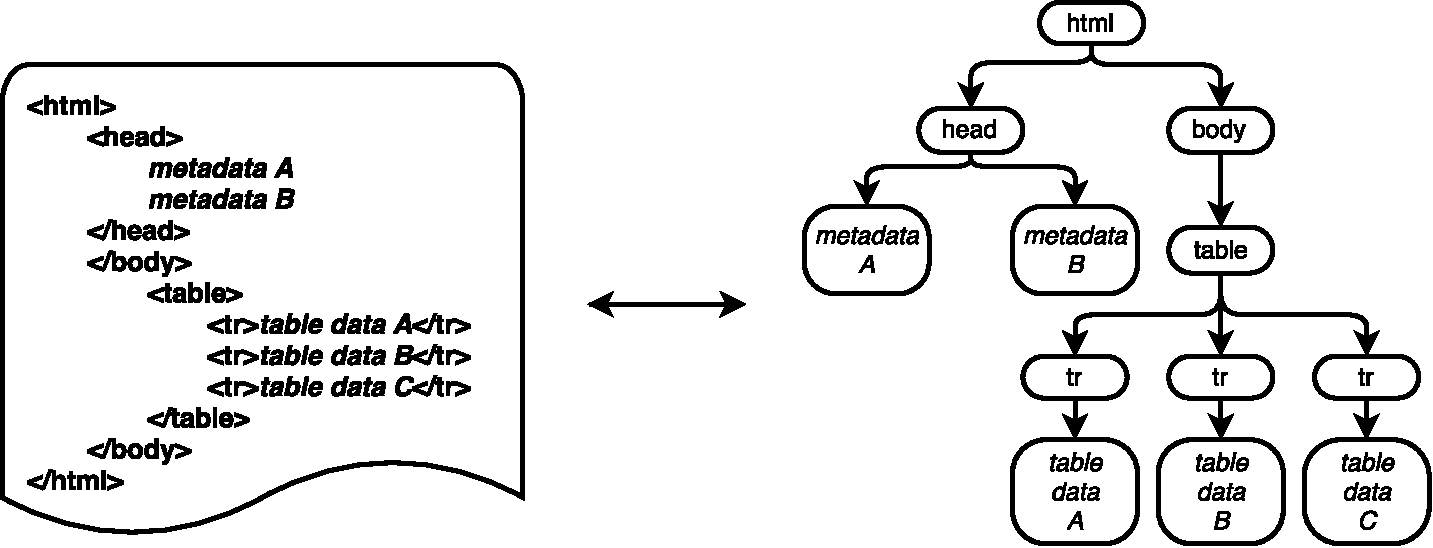
\includegraphics[width=\textwidth]{Data_Acquisition/html_tree.pdf}
    \caption[Tree representation of HTML Code]{Tree representation of HTML code. The html code here displays a table with three rows. The page has two pieces of meta-data associated with it, stored in the `head'.}
\label{fig:HTMLTREE}
\end{figure}
XPaths are just paths through the document tree to the desired information. In order the `scrape' the data in the table, the following XPath could be used:
\begin{center}
\texttt{//html/body/tr/*}
\end{center}
This presents an immediate problem, as scraping a millions of webpages requires millions of potentially different XPaths to be known. It is impractical to specify them manually, thus the challenge of large-scale scraping is how to identify and collect useful data on webages without manually specifying many XPaths.
\section{Automatic XPath Generation}
The initial approach was to analyse the HTML tree to automatically recognise useful tabulated or listed data. The program started at the tree's root and repeatedly followed the branch with the most `repeating substructure'. The recursive algorithm is summarised below:
\begin{sloppypar}
\begin{enumerate}
\item \texttt{Count \# of descendents of each child node}
\item \begin{enumerate}
\item \texttt{Calculate the pairwise similarities between all child nodes}
\item \texttt{Consider  two nodes similar if pairwise similarity is above a heuristic threshold}
\item \texttt{Calculate proportion of nodes that are considered similar}
\end{enumerate}
\item \texttt{If proportion calculated in (c) is above a heuristic threshold, this node represents a store of information, and the XPath has been found. Otherwise, move to child node with highest \# of descendants, return to step (1)}
\end{enumerate}
\end{sloppypar}
The heuristic thresholds are adjustable parameters. The approach was successful for webpages with large numbers of records, formatted in repeating fashion, but performed poorly for smaller collections of data. As such it was not sufficiently flexible for the task of scraping large quantities of chemical data, and was not developed further.
\section{Collection Strategy}
As generating XPaths proved unsuitable, a new strategy was required. Chemical information is usually disseminated as journal articles, mostly accompanied by a DOI. By programmatically collecting DOIs, (\S\ref{sec:DOI}) it was possible to build up a large database of chemical information (see  \S\ref{sec:SCRAPING_PROGRAM})
\subsection{DOIs : Document Object Identifiers}
\label{sec:DOI}
DOIs are computer-friendly labels for articles. DOIs are issued by a number of accredited bodies, with the vast majority of chemistry-related articles issued by Crossref.\footnote{Crossref is a not-for-profit body comprised from Publishers International Linking Association (PILA), an association of many academic publishers} \cite{crossref-formation}. By pre-pending a DOI string with the url stub \texttt{http://dx.doi.org/}, the International DOI foundation (IDF) service redirects the request to the publisher's website to display the article the DOI refers to. The structure of a DOI is shown in Figure \ref{fig:DOI}.
\begin{figure}[H]
    \centering
    \textbf{Anatomy of a DOI}\par\medskip
    \includegraphics[width=\textwidth]{Data_Acquisition/DOI2.png}
    \caption[Anatomy of a DOI]{DOI structure. The structure consists of a numeric prefix (X and Y must be integers) and alphanumeric suffix (Z can be any Unicode-encoded character)} \label{fig:DOI}
\end{figure}
DOIs consist of a prefix and a suffix. The prefix is subdivided into the ‘Directory Indicator’ (always integer ‘10’) separated from the ‘Registrant Code’, assigned by the issuing body \cite{doi_handbook1}. Registrant codes are numeric and can be a minimum of three integers, with further optional subdivisions separated by full stops. The suffix is provided by the registrant themselves and can be any form of unicode-encoded text \cite{doi_handbook1}.


It was possible to write a `Regular Expression' pattern matcher (regex) to automatically recognise DOIs within a body of text (see Figure \ref{fig:REGEX}). The flexibility of the registrant code specification means that DOIs cannot always be unambiguously identified in HTML documents. 
\begin{figure}[H]
    \centering
    \textbf{Pattern Matching Procedure for DOIs}\par\medskip
    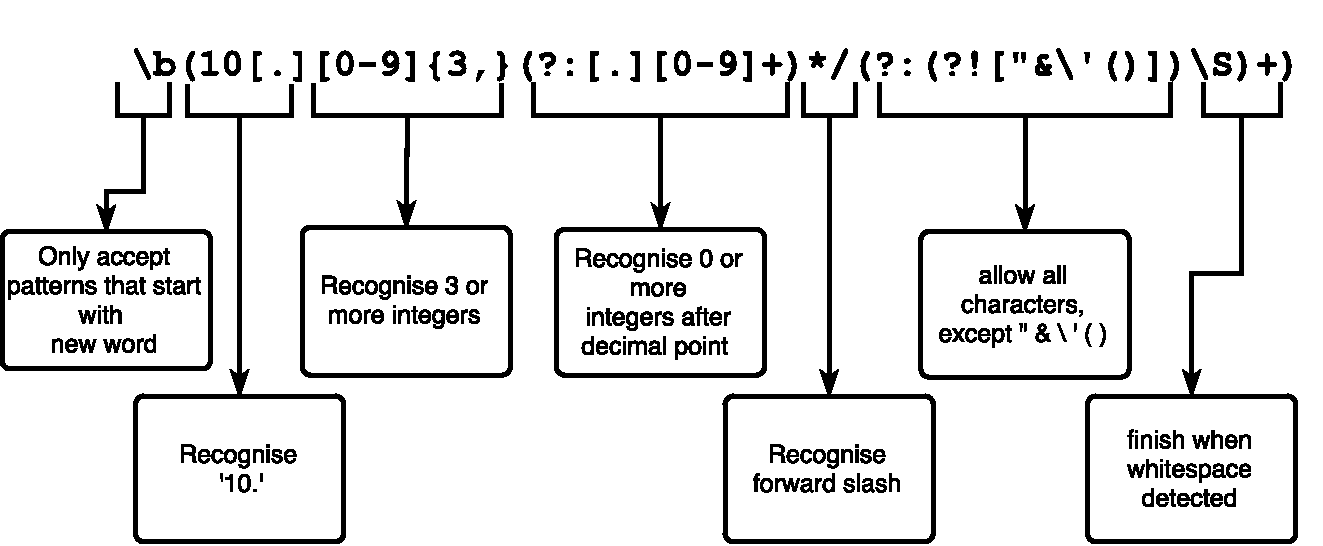
\includegraphics[width=\textwidth]{Data_Acquisition/Regex.pdf}
    \caption[Pattern Matching Procdure for DOIs]{Perl Syntax Regex Code that can identify the vast majority of DOIs within free text)} \label{fig:REGEX}
\end{figure}
Despite this, the regex was able to identify 90.4\% of the dois on the Cambridge University Chemistry Department website \url{http://www.ch.cam.ac.uk/publications}. 
\subsection{Scraping Program}
\label{sec:SCRAPING_PROGRAM}
The Regex approach does not require XPaths in order to extract DOIs from a webpage. This facilitates large scale scraping from a large set of websites. Some meta-data associated with a DOI can be accessed using an online API exposed by Crossref. Further metadata can be accessed by following the \texttt{http://dx.doi.org/\{DOI\}} redirecting service by DOI$^{\circledR}$.org. to visit publishers' websites to collect remaining meta-data. 

With this methodology in place, a scraping program was written to collect DOIs from a list of webpages and collect meta-data in a two stage process. The Crossref API provides article titles, journals, authors, publisher and publication date meta-data, but not article abstracts. These had to be collected by visiting publisher webpages, and collecting with hand written XPaths\footnote{Since there are comparatively few publisher websites, only 26 publisher XPaths were required for decent capture coverage.}. The procedure is summarised in figure \ref{fig:Cherry}.
\begin{figure}[H]
    \centering
    \textbf{Scraping Procedure}\par\medskip
    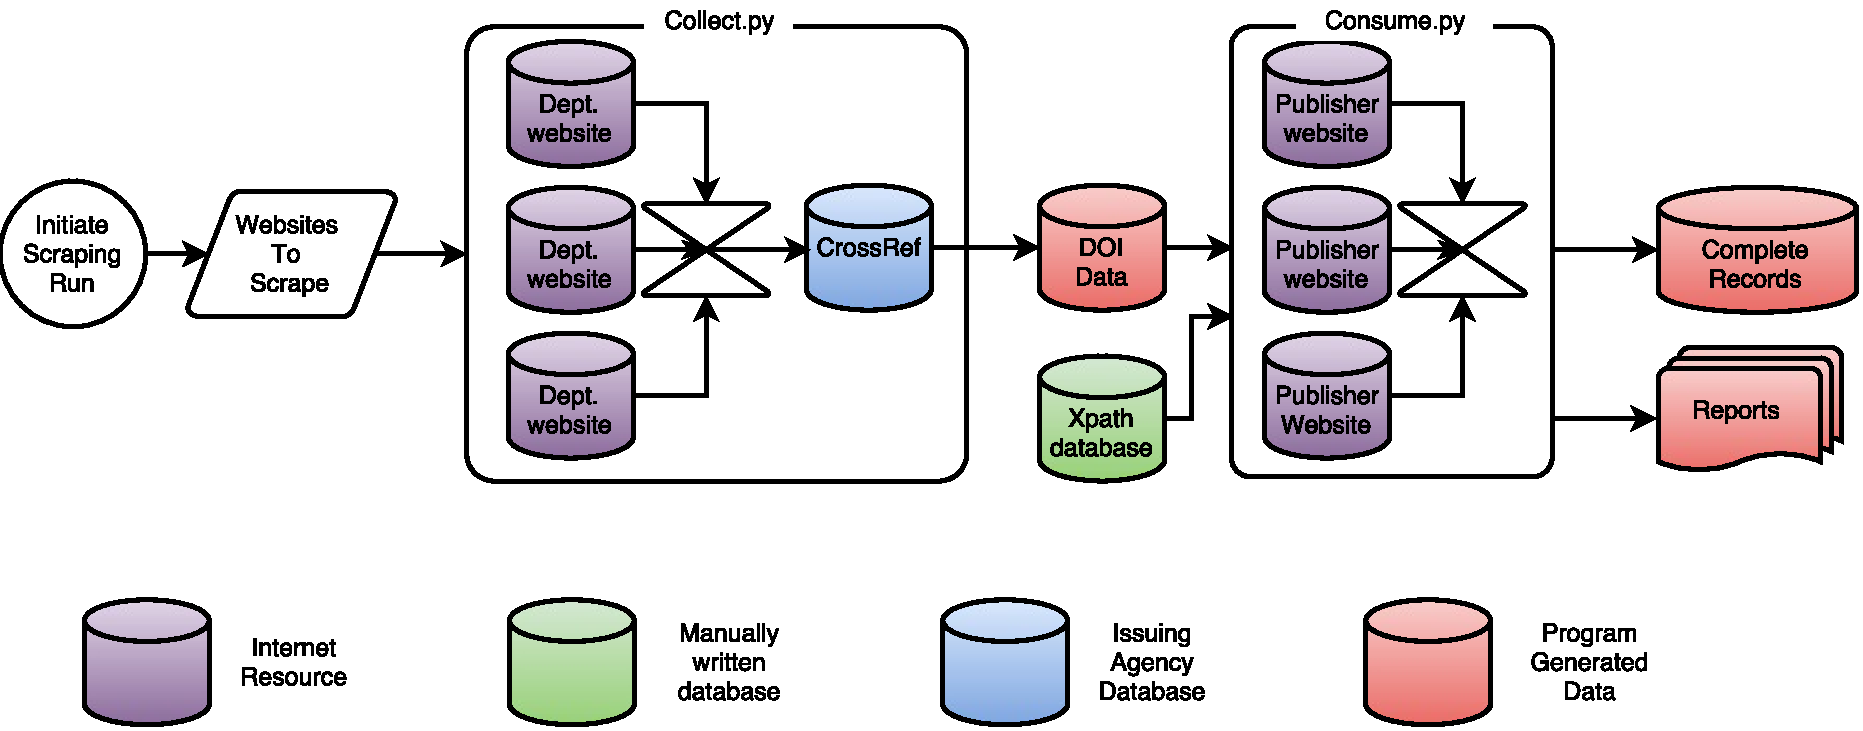
\includegraphics[width=\textwidth]{Data_Acquisition/Cherry2.pdf}
    \caption[Data Flow in Scraping Procedure]{The data flow of the scraping program. Websites from an inputted list of websites are visited and DOIs are extracted in the process described in  \S\ref{sec:DOI}. The Crossref API service is then used to verify the extracted DOIs, and collects available meta-data. The program then accesses publisher webpages and collects abstracts. The program also produces explanation of capture failures and some general statistics}
\label{fig:Cherry}
\end{figure}
The programmatic steps depicted in figure \ref{fig:Cherry} are:
\begin{sloppypar}
\begin{enumerate}
\item \texttt{Request the webpage from the inputted list}
\item \texttt{Process the html and extract DOIs}
\item \texttt{Using the Crossref Online API, verify the extracted DOIs exist}
\item \texttt{Crossref yields metadata:}
\begin{itemize}
\item \texttt{Title}
\item \texttt{Journal}
\item \texttt{Publisher}
\item \texttt{Authors}
\item \texttt{Publication Date}
\end{itemize}
\item \texttt{For each DOI,  follow \texttt{http://dx.doi.org/\{DOI\}} link}
\item \texttt{Use XPath to collect article abstracts}
\end{enumerate}
\end{sloppypar}
The program exports complete records as .json files, but also feeds directly to a MongoDB database. Once the program was written, the next priority was to obtain a list of webpages to scrape. This is described in  \S\ref{sec:UKSCRAPE} and \S\ref{sec:CROSSREFSCRAPE} 
\section{Collection Results}
\subsection{UK University Department scraping}
\label{sec:UKSCRAPE}
The program was first used to collect the data from the UK. The Goodman group's website hosts a list of UK chemistry departments \url{http://www-jmg.ch.cam.ac.uk/data/c2k/uk.html}. The list was manually checked and some URLs were changed to give a list of 68 departments\footnote{Details can be found in the appendix}. The program was run with this list as input, the results of which are detailed in table \ref{tab:UKSCRAPERES}. The DOIs collected were stored in database $\Delta1$ and the complete results were stored in database $\Delta2$.
\begin{table}[h!]
\caption{UK Scraping results}
\label{tab:UKSCRAPERES}
\begin{center}
\begin{tabular}{||l|l|l||}
\hline
Process & \# records & \% of maximum yield\\
\hline
Dois collected & 22442 & N/A\%\\
Dois found with metadata & 22397 & 99.8\%\\
Articles successfully resolved & 16363 & 72.9\%\\
Losses due to failed requests & 2753 & 12.3\%\\
Program errors & 133 & 0.6\%\\
Missing Publication Errors & 3148 & 14.0\% \\
\hline
\end{tabular}
\end{center}
\end{table}
Conversion losses were due to four components. 45 losses for non-existant DOIs, 2753 losses to request errors (404 : not-found errors or permission problems), 133 to the program errors and 3148 conversions were lost due missing publication XPaths. The 26 specified XPaths \footnote{Corresponding to 37 publishers} were sufficient to convert 83.8\% of successful requests. This was deemed acceptable, as most major publishers had been covered\footnote{see appendix for list of covered publishers}, and the missing publishers each covered a small number of articles\footnote{It would take another 11 XPaths of the missing most popular publishers to increase the conversion rate from 83.8\% to 90\%.}
The efficiency is depicted in figure \ref{fig:UKSANK}.

\begin{figure}[H]
    \centering
    \textbf{Efficiency of UK Department Scraping}\par\medskip
    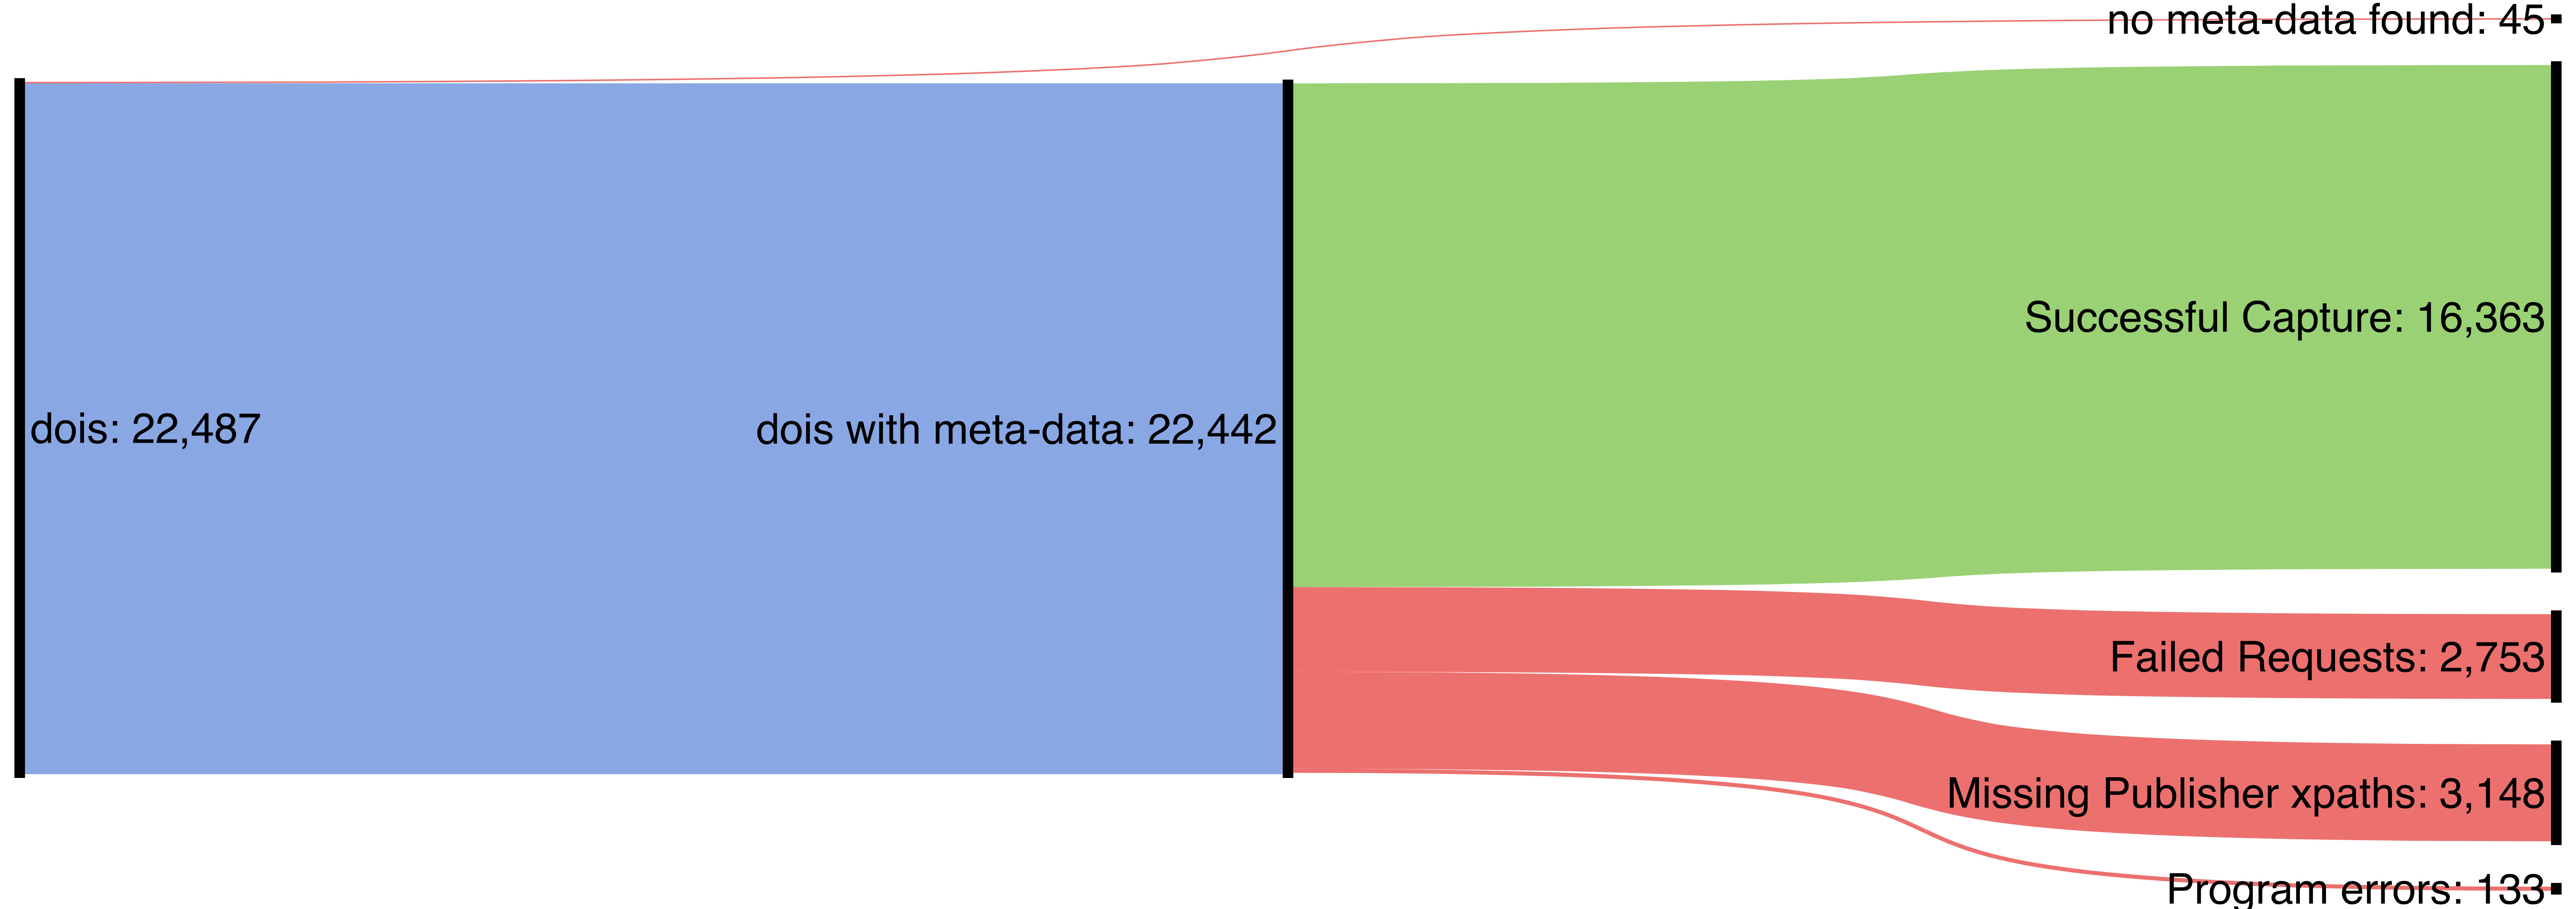
\includegraphics[width=\textwidth]{Data_Acquisition/uk_sankey.png}
    \caption[Efficiency of UK Department Scraping]{The loss processes are coloured red, successfully captured full records in green, and the maximum possible yield in blue.}
     \label{fig:UKSANK}
\end{figure}

Interestingly, 9467 out of 16363 successful collections were sourced from \url{http://www.ch.cam.ac.uk}. This could be because the department at Cambridge has an extensive website and also hosts the majority of its information under its own domain name, whereas other departments' data are hosted on central university domains. The scraping program was confined to scrape only webpages belonging directly to chemistry department domains, not the university website as a whole. As a result, it is worth bearing in mind that the Cambridge chemistry department may be overrepresented in the UK chemistry data set.

\subsection{Global Scale Scraping}
\label{sec:CROSSREFSCRAPE}
Much more data would be required to train a successful machine learning model. One approach would have been to expand the scrape to world-wide chemistry departments, and other learn\`{e}d bodies. However, Crossref also exposes a search service that can be used to query its vast internal database. The program was then set up to query the Crossref service for search terms `Chemistry', `Chemical', `Molecule' and `Molecular' for journal articles and journal titles. This suggested possible yields in the millions of articles. 

The program was instructed to scrape the search results pages of these queries. Because the scraping job was large, it was programmed to `pause' before publisher abstract collection. The results up to this point were examined before setting off the second stage to collect abstracts.

At the intermediate point, the program had collected 1,267,495 records, which would provide enough data to train a powerful machine learning algorithm. This database was labelled $\Delta3$.

The publisher distributions were then considered\footnote{Some of this analysis is presented in \S\ref{sec:SCRAPEANALYSIS}.}. After careful considerations of request server loads and predicting capture probabilities, the second half of the scraping routine was set off to run for three days.
\label{sec:CROSSREFSCRAPE}
\subsection{Problems with ACS and Taylor \& Francis}
\label{sec:banning1}
Most publishers track request volumes sent to their servers to discourage automatic downloading. However, scraping constitutes fair use and complies to UK copyright law. Despite the university owning a full-access licence to these publishers' publications, the collected material was freely available without licence\cite{thelaw} \cite{contentminelegal}. During the scraping run, a bug in the randomisation of requests resulted in detection by ACS and Taylor \& Francis, which responded by banning the scraping computer's IP address (Explored further in \S\ref{sec:banning2}). The department librarians were able to restore access, and it was agreed that no further scraping would be performed.
\subsection{Analysis of collected data}
The yield of the global-scale scraping run was cut significantly by the ACS banning event. A summary is tabulated in table \ref{tab:LARGESCRAPERES} and shown graphically in figure \ref{fig:LARGESANK}. The complete records were stored in a database $\Delta4$.
\begin{table}[h!]
\caption{Global Scraping Results}
\label{tab:LARGESCRAPERES}
\begin{center}
\begin{tabular}{||l|l|l||}
\hline
Process & \# records & \% of maximum yield\\
\hline
DOIS collected &  1267495 &N/A\\
DOIS collected with meta-data &  1267495 &100.0\%\\

\hline
Predicted maximum capture & 1071506 &  84.5\%\\
Predicted Capture without ACS & 581797 & 45.9\%\\
\hline
Articles successfully captured & 714370 & 56.4\%\\
Losses to failed requests (excluding ACS)& 53743 & 4.2\%\\
Losses to ACS banning & 303393 & 23.9\%\\
Missing Publications \& Program Errors & 195989 & 15.5\%\\
\hline
\end{tabular}
\end{center}
\end{table}
\begin{figure}[H]
    \centering
    \textbf{Efficiency of Global Scraping}\par\medskip
    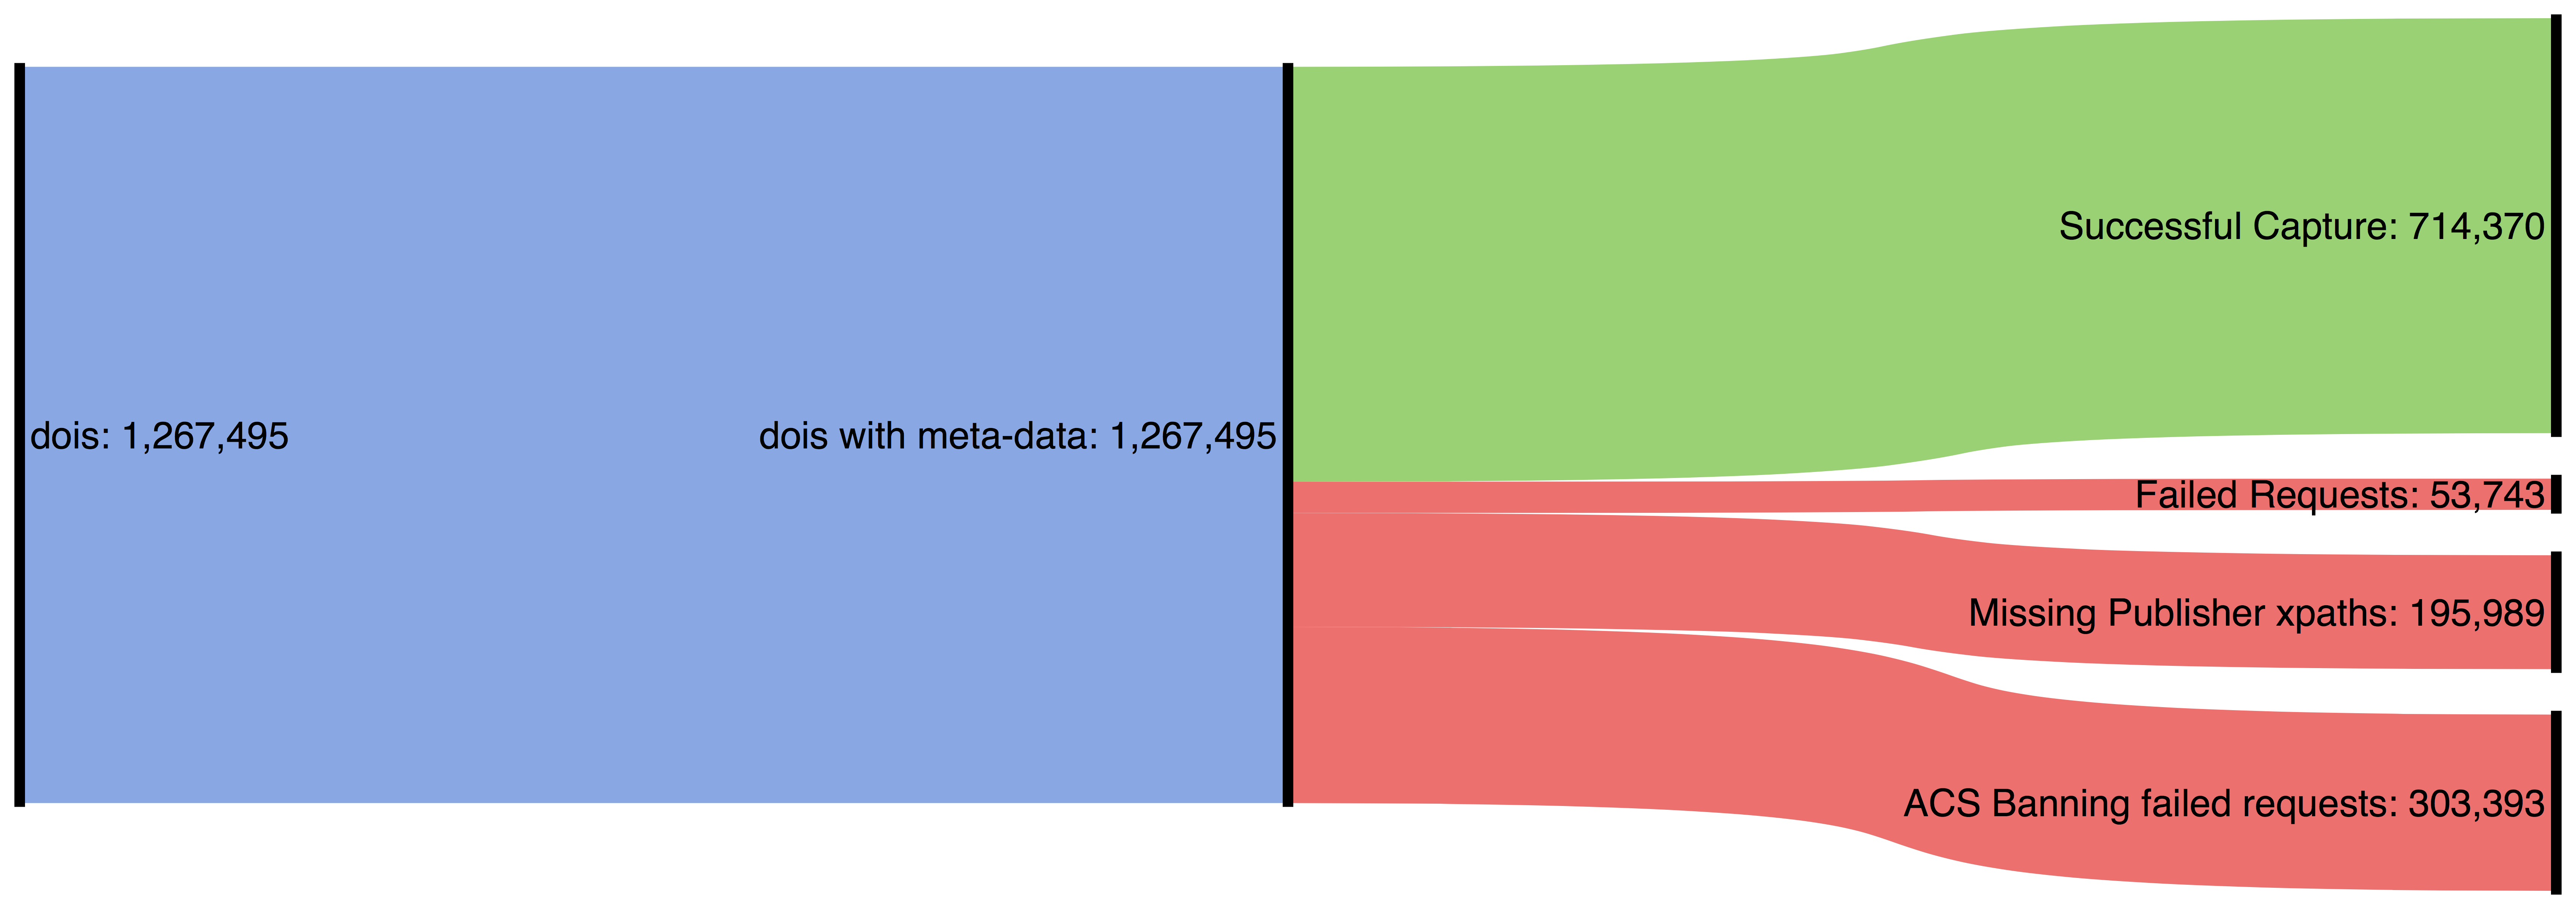
\includegraphics[width=\textwidth]{Data_Acquisition/large_sankey.png}
    \caption[Efficiency of Large Scale Scraping]{The loss processes are coloured red, successfully-captured full records in green, and the maximum possible yield in blue.}
     \label{fig:LARGESANK}
\end{figure}

The overall efficiency of the process is 56.4\%, but excluding lost ACS records, the program's efficiency jumped to 74.0\%, similar to the efficiency of the UK scraping run (\S\ref{sec:UKSCRAPE}). \footnote{Also note that 100\% of DOIs were converted to DOIs with meta-data. This is because the format of the webpages scraped was consistent for every DOI collected.}

The successfully captured 714,370 records merged with the UK results\footnote{The merged Dataset was labelled $\Delta5$}. Records were rejected with short titles or abstracts, or if the majority of the title and abstract were not written in ascii characters\footnote{likely to be addenda, informal articles, retractions etc, and removing removing majority Japanese and Chinese script}. This was done to provide higher-quality data for training the algorithm (see \S\ref{chapt:ALGORITHM}). This filtering resulted in a final training database of 464712 articles. This dataset was labelled $\Delta6$. The entire database formation process is shown in figure \ref{fig:DATABASES} and table \ref{tab:DATABASES}.
\begin{figure}[H]
    \centering
    \textbf{Summary of Database Preparation}\par\medskip
    \includegraphics[scale=0.6]{Data_Acquisition/Databases2.pdf}
    \caption[Summary of Database Preparation]{Blue databases ($\Delta1$, $\Delta3$) represent data with DOIs and meta-data. Green databases ($\Delta2$, $\Delta4$ ) represent meta-data, DOIs and abstracts. The purple database ($\Delta5$) is the combined complete records, and the red database is the data deemed suitable for the training algorithm. Database Populations and losses are annotated.}
     \label{fig:DATABASES}
\end{figure}
\begin{table}[H]
\caption{Databases created in Data Acquisition Process}
\label{tab:DATABASES}
\begin{tabular}{||c|c|c|c||}
\hline 
Database &  Contents & \# Records\\
$\Delta1$ & Dois found on UK Chemistry Department websites & 22,397 \\
$\Delta2$ & Complete meta-data obtained from records in $\Delta1$ & 16,363 \\
$\Delta3$ & Dois found in global scraping using crossref API & 1,267,495  \\
$\Delta4$ & Complete meta-data obtained from records in $\Delta3$ & 714,370 \\
$\Delta5$ & Complete records obtained from combining $\Delta2$ and $\Delta4$ & 730,733 \\
$\Delta6$ & Records appropriate for training taken from $\Delta5$ & 464,712 \\
\end{tabular}
\end{table}


It was instructive to examine these databases and derive some simple statistical results, explored in \S\ref{sec:CORPUSOBSERVATIONS}.
%\chapter{Techniques for Language Processing}
\section{Background}
To Do
\section{Bag of Words}
To Do
\section{Bag of Citations}
To Do
\section{Word2Vec}
To Do
\section{Doc2Vec}
To Do
%\chapter{Algorithm Development}
\label{chapt:ALGORITHM}
\section{Premise}
To Do
\section{Data Sanitisation}
To Do
\section{Word2Vec Models}
To Do
\subsection{Aggregation Techniques}
To Do
\section{Doc2Vec Models}
To Do
%\chapter{Model Examination}
\label{chapt:VALIDATION}
The models created in \S\ref{chapt:ALGORITHM} were then examined and assessed. As an unsupervised learning algorithm, it is challenging to assess model quality, due to a lack of concrete metrics for comparisons\footnote{This is to say, there is no objective `similarity' relationship value between two words to compare models to.}. The Word2Vec development team tested with approximately 10,000 semantic and syntactic relationships (See Figure \ref{fig:KINGQUEEN})\cite{word2vec1},\cite{word2vec2},\cite{word2veckingqueen}. The scope of this project does not extend to such elaborate tests. In the section, some examples of model strengths are given and techniques for using word vectors and visualisation are presented. 
\section{Word Similarities}
Word similarities can be be obtained by direct comparison of their word vectors. A possible metric is to compute euclidean distance.  For words $\alpha$ and $\beta$, with vectors $\mathbf{\nu^\alpha}$ and $\mathbf{\nu^\beta}$, 

$$S_{euclid} = \sqrt{\sum_{i=1}^{D}(\nu_i^{\alpha}-\nu_i^{\beta})^{2}} $$

where $D$ is the dimensionality ($D$=100). $S_{euclid}$ simply describes the distance between the end points of $\mathbf{\nu^\alpha}$ and $\mathbf{\nu^\beta}$. A larger $S_{euclid}$ indicates weaker similarity. A second similarity metric is \emph{cosine similarity}, a measure of the directionality. A value close to 1 corresponds to high similarity of $\alpha$ and $\beta$. Cosine similarity is computed as:
$$S_{cosine}=\frac{\mathbf{\nu^\alpha} \cdot \mathbf{\nu^\beta}}{|\mathbf{\nu^\alpha}| |\mathbf{\nu^\beta}|} = \frac{\displaystyle\sum_{i=1}^{D} \nu^{(\alpha)}_{i}\nu^{(\beta)}_{i}}{\left(\displaystyle\sum_{i=1}^{D} (\nu^{(\alpha)}_{i})^2\right)^{1/2} \left(\displaystyle\sum_{i=1}^{D} (\nu^{(\beta)}_{i})^2\right)^{1/2}}
$$
The CBOW and skipgram models were examined using these metrics. For a given word, the models were requested to return the three words in the corpus with highest similarity. Some examples are given in tables \ref{tab:COSINESIMS} and \ref{tab:EUCLIDSIMS}.
\begin{table}[H]
\begin{center}
\caption[Word similarity examinations with cosine similarity]{Closest words to test words using cosine similarity}
\label{tab:COSINESIMS}
\begin{tabular}{||c||c|c|c|c||}
\hline
Model     & Test Word              & Most Similar & 2nd & 3rd \\ \hhline{||=||=|=|=|=||}
CBOW      & \multirow{2}{*}{Iron} & Chromium             &  Manganes   &   Nickel  \\ \cline{1-1} \cline{3-5} 
Skip-gram &                   &  Chromium            &   Manganes  &  Nickel   \\ 
\hhline{||=||=|=|=|=||}
CBOW      & \multirow{2}{*}{Colloid} & Nanoparticl             &  Nanos   &   Monodispers  \\ \cline{1-1} \cline{3-5} 
Skip-gram &                   &  Particl            &   Spheric  &  Suspens   \\ 
\hhline{||=||=|=|=|=||}
CBOW      & \multirow{2}{*}{Statistical} & Varianc             &  Bayesian   &   Multivari  \\ \cline{1-1} \cline{3-5} 
Skip-gram &                   &  Nonparametr            &   Varianc  &  Bootstrap   \\ 
\hhline{||=||=|=|=|=||}
CBOW      & \multirow{2}{*}{Plastic} & Thermoplast             &  Elastomer   & Nonwoven    \\ \cline{1-1} \cline{3-5} 
Skip-gram &                   &  Nonwoven            &   Thermoplast  &  Textolit   \\ 
\hhline{||=||=|=|=|=||}
CBOW      & \multirow{2}{*}{Catalyst} & Cocatalyst             &  Nanocatalyst   & Precatalyst    \\ \cline{1-1} \cline{3-5} 
Skip-gram &                   &  Catalyt            &   Nanocatalyst  &  Polystyrylbipyridin   \\ 
\hhline{||=||=|=|=|=||}
\end{tabular}
\end{center}
\end{table}

\begin{table}[h!]
\begin{center}
\caption[Word similarity examinations with euclidean similarity]{Closest words to test words using Euclidean similarity}
\label{tab:EUCLIDSIMS}
\begin{tabular}{||c||c|c|c|c||}
\hline
Model     & Test Word              & Most Similar & 2nd & 3rd \\ \hhline{||=||=|=|=|=||}
CBOW      & \multirow{2}{*}{Iron} & Chromium             &  Managanes   &   Nickel  \\ \cline{1-1} \cline{3-5} 
Skip-gram &                   &  Chromium            &   Manganes  &  Nickel   \\ 
\hhline{||=||=|=|=|=||}
CBOW      & \multirow{2}{*}{Colloid} & Nanos             &  Ultrafin   &   Agglomer  \\ \cline{1-1} \cline{3-5} 
Skip-gram &                   &  Particl            &   Suspens  &  Spheric   \\ 
\hhline{||=||=|=|=|=||}
CBOW      & \multirow{2}{*}{Statistical} & Varianc             &  Phenomenolog   &   Bayesian  \\ \cline{1-1} \cline{3-5} 
Skip-gram &                   &  Nonparametr            &   Bivari  &  Multigrid   \\ 
\hhline{||=||=|=|=|=||}
CBOW      & \multirow{2}{*}{Plastic} & Thermoplast             &  Elastomer   & Mold    \\ \cline{1-1} \cline{3-5} 
Skip-gram &                   &  NRL            &   Prepreg  &  Sealant   \\ 
\hhline{||=||=|=|=|=||}
CBOW      & \multirow{2}{*}{Catalyst} & Nanocatalyst             &  Cocatalyst   & Precatalyst    \\ \cline{1-1} \cline{3-5} 
Skip-gram &                   &  Catalyt            &   Molybdena  &  Nimo   \\ 
\hhline{||=||=|=|=|=||}
\end{tabular}
\end{center}
\end{table}
As shown above, the models perform well, returning intuitively similar words to the test word.\footnote{Note that returned words are 'stemmed' from use of stemming algorithm before training. It is not difficult to interpret derived words from their stems.}. In most cases, chemical inference is represented in some way\footnote{e.g. the models understood that catalysts and nanocatalysts are closely-connected concepts.}.

It was observed that the skipgram model gave misleading positives more frequently\footnote{in the catalyst case above, skipsgram associated a stemming false negative and gave a specific catalysed compound to the `catalyst' test word than more obvious, fundamental associations.}. CBOW  was considered to be superior for word-word comparisons. It was also noted that CBOW had closer agreement between $S_{euclid}$ and $S_{cosine}$, however, euclidean similarity gave poorer general performance.\footnote{`NRL' in the `Plastic' category of skip-gram is a typical example of poorer euclidean performance. NRL appears to be a reference to the Navy Reseach Laboratory. }. It was noted that $S_{cosine}$ is the accepted similarity metric in the literature \cite{word2vec1},\cite{word2vec2},\cite{doc2vec}.

\section{Document Similarities}
The models detailed in \S\ref{chapt:ALGORITHM} were then tested for document vector similarity. A document was chosen from the corpus, the three most similar articles were computed for each model and results assessed. One test document was \texttt{DOI: 10.1134/s0036024412120266} \cite{docassay}:


\texttt{`Photochemical transformations of anthraquinone in polymeric alcohols'}.

 The TF-IDF models (CBOW-TFIDF-S, CBOW-TFIDF-W, SG-TFIDF-S, SG-TFIDF-W) suffered from mathematical conditioning problems, giving poor predictions. The remaining models' most similar documents \footnote{Cosine similarity was used, as it performed better than euclidean similarity for document vectors.} for this test document are shown in table \ref{tab:DOCSIMS}:
\begin{table}[H]
\centering
\caption[Examination of Document Vector similarities]{Document Vector Similarities to \cite {docassay}}
\label{tab:DOCSIMS}
\begin{tabular}{|l|p{2cm}|p{4cm}|p{2cm}|p{4cm}|}
\hline
Model           & DOI            & Title            & DOI              & Title              \\ \hline
CBOW-W               & 10.1080/ 00222338 208074396         & \footnotesize{Oxidation of Poly(dimethylbutadiene) Popcorn Polymer} &  10.1246/ cl.1974.133               &                   \footnotesize{photochemical reaction of 2-cyanoquinoline 1-oxides in an acidic alcohol. synthesis of 6-alkoxy-2-cyanoquinolines} \\ \hline
CBOW-S               & 10.1002/ pol.1985 .170230401          &  \footnotesize{Polymerization of glycidol and its derivatives: A new rearrangement polymerization}
                & 10.1080/ 002223381 08074381                & \footnotesize{Cyclic Acetal-Photosensitized Polymerization. 9. Photopolymerization of Triallylidene Sorbitol}
                   \\ \hline
SG-S                 & 10.1002/ pola.1991. 080290207            &   \footnotesize{Photochemical synthesis of nitroxyl free radicals in the presence of vinyl monomers}
               &  10.1002/ pola.10311              &  \footnotesize{Benzyl alcohols as accelerators in the photoinitiated cationic polymerization of epoxide monomers}
                  \\ \hline
SG-W                 & 10.1080/ 00222338 208074396            &    \footnotesize{Oxidation of Poly(dimethylbutadiene) Popcorn Polymer}
              & 10.1080/ 00222338 408077237                &  \footnotesize{Photopolymerization of Acrylonitrile: Benzophenone-Isopropanol System as Initiator}
                 \\ \hline
doc2vec                    &  10.1002/ pola.10059              &  \footnotesize{Aqueous photopolymerization with visible-light photoinitiators: Acrylamide polymerization photoinitiated with a phenoxazine dye/amine system}
                & 10.1080/ 10587259 408029732                 & \footnotesize{ An Investigation into the Solid-State Behaviour of Anthraquinone and Its Derivatives}
                 \\ \hline
\end{tabular}
\end{table}
The document vectors generated by the Doc2Vec model had considerably better general performance, and were selected as the model of choice for further analysis.  
\section{Visualisation Techniques}
\subsection{Network Visualisation}
High Dimensional systems are difficult to visualise but there are several methods available to visualise high-dimensional data. PCA\footnote{See Glossary} \cite{PCA} and TSNE\footnote{See Glossary}\cite{tsne1},\cite{bhtsne} techniques allow 100-dimensional document vectors to be collapsed to points on an arbitrary 2D plane, to give a visual `snapshot' of the semantic space. 
Figures \ref{fig:PCA_snap} and \ref{fig:TSNE_snap} show PCA and TSNE reductions on 10,000 document vectors randomly selected from the Doc2Vec model representation of $\Delta6$\cite{scikitlearn}.

\begin{figure}[H]
  \centering
  \begin{minipage}[b]{0.49\textwidth}
	\begin{center}\textbf{PCA Dimensional Reduction}\end{center}
    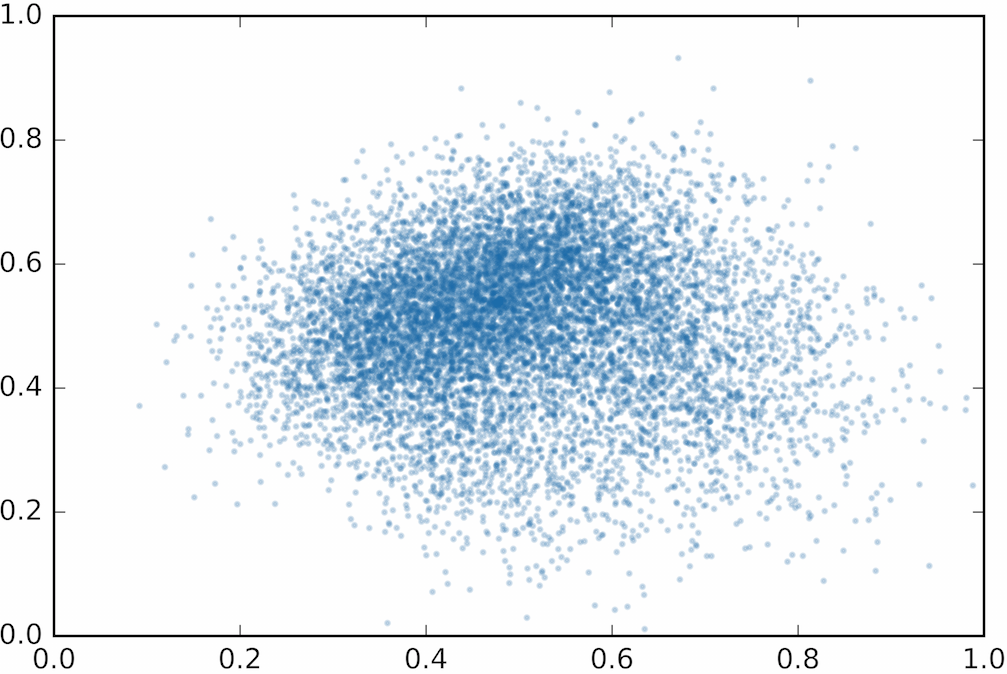
\includegraphics[width=\textwidth]{Validation/pca2.png}
    \caption[PCA Dimensional Reduction]{PCA map of 10,000 documents in the corpus. PCA has not resolved any particular structure. The dimensional reduction task is probably too challenging for PCA.\\ \\ \\ \\}
      \label{fig:PCA_snap}
  \end{minipage}
  \hfill
  \begin{minipage}[b]{0.49\textwidth}
  \begin{center}\textbf{TSNE Dimensional Reduction}\end{center}
    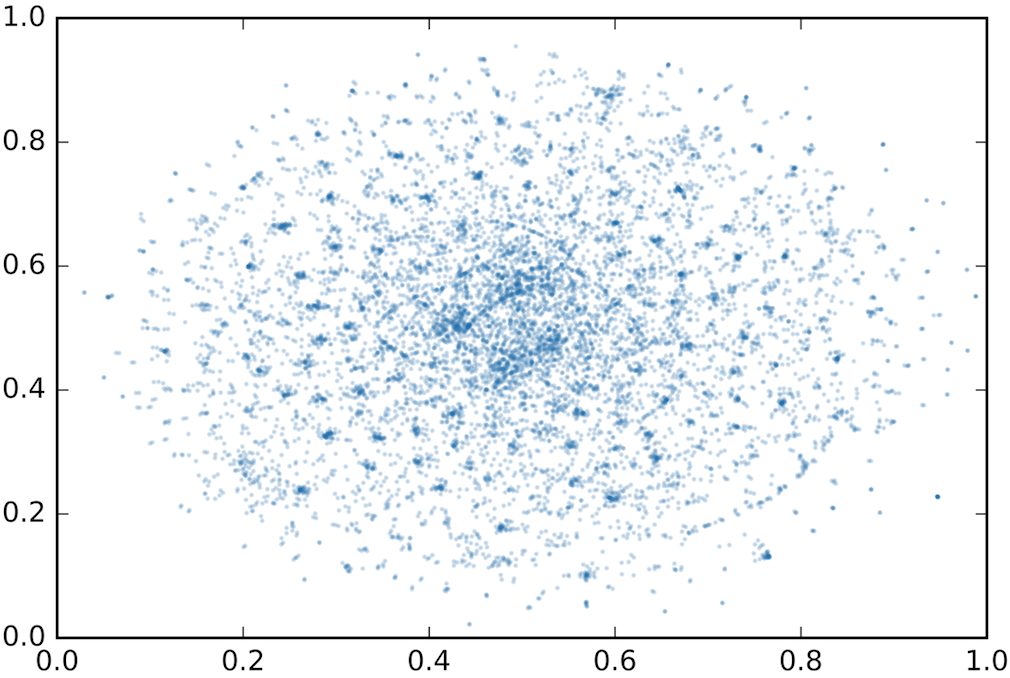
\includegraphics[width=\textwidth]{Validation/tsne2.png}
    \caption[TSNE Dimensional Reduction]{TSNE map of the same 10,000 documents. TSNE is a much more sophisticated, state of the art technique, that seeks to preserve high dimensional clusters. Document vectors have gathered into noticeable clusters, with non negligible outlier documents between clusters. Performed using Barnes-Hut TSNE implementation as sample size is large. }
      \label{fig:TSNE_snap}

  \end{minipage}
\end{figure}
The PCA reduction shows a dark central area, suggesting most vectors are `smeared' about a common direction. The map is not symmetric which is what would be expected for random vectors. It was expected that document vectors would be distributed in clusters representing particular research fields within the literature. This is indeed seen in the TSNE reduction, which resolved many clusters. There are document vectors scattered between dark cluster spots, which may be could interpreted as `interdisciplinary'\footnote{More in-depth analysis of TSNE maps forms part of the recommended work section, \S\ref{chapt:RECOMMENDATIONS}}.
TSNE is based upon euclidean distance, which is noted not to be the best similarity measure. Whilst qualitatively useful, TSNE maps were interpreted cautiously.
\subsection{Networks and Network Visualisation}
\label{sec:COSINEMAT}
A $S_{cosine}$ matrix $\mathbf{C}$ was defined between sets of documents. For a set of documents  A (with $a$ documents) and B (with $b$ documents) document matrices of document vectors were defined, $\mathbf{A}$ and $\mathbf{B}$, such that 

$$\mathbf{A} = \left( \begin{array}{cccc}
\vdots & \vdots & \vdots & \vdots \\
\mathbf{w}_1 & \mathbf{w}_1 & \cdots & \mathbf{w}_a \\
\vdots & \vdots & \vdots & \vdots \\ \end{array} \right) , \mathbf{B} = \left( \begin{array}{cccc}
\vdots & \vdots & \vdots & \vdots \\
\mathbf{v}_1 & \mathbf{v}_1 & \cdots & \mathbf{v}_b \\
\vdots & \vdots & \vdots & \vdots \\ \end{array} \right)$$ where $w$ and $v$ are document vectors.
$\mathbf{C}$ was then defined as $\mathbf{C}_{i , j} = cosine \left(\theta_{i , j} \right)$ where element i,j contains the cosine between $i$th vector in A and $j$th vector in B:
$$\mathbf{C}_{i , j}=\cos(\theta_{i ,j}) \ \ \ \ \ \mathbf{C}=\mathbf{A}^T \mathbf{B} \oslash \left( diag(\mathbf{A}^T \mathbf{A})^T diag(\mathbf{B}^T \mathbf{B}) \right)^{\circ\frac12}$$
where $\oslash$ and $^{\circ\frac12}$ indicate Hadamard division and Hadamard square root, $diag(Q)$ the $1 \times n$ matrix formed from the diagonal of $Q$. $\mathbf{C}$ represents a network where each document in A is a node with an edge to every document in B with weights equal to the cosine. If A=B, then the matrix is a fully connected network\footnote{That is to say, if A and B are the same set of documents, every document node has an edge to every other document in the set}. This network can be visualised using specialist software\footnote{Gephi, a powerful, open source network visualisation and analysis suite, was used for this purpose. }\cite{gephi}. Figure \ref{fig:gephi_exp} visualises the same 10,000 document sample as a network graph.
\begin{center}
\begin{figure}[H]
  \centering
  \textbf{Network Visualisation of 10,000 document sample}
     \makebox[\textwidth][c]{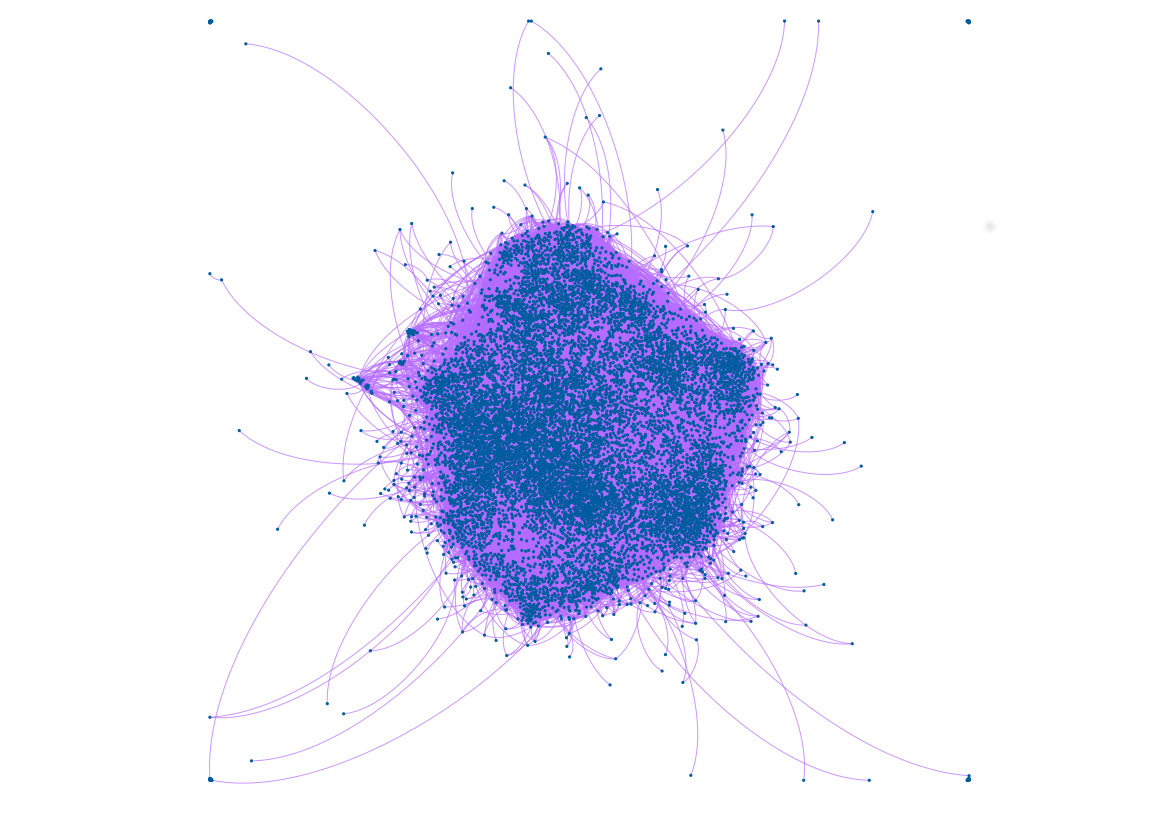
\includegraphics[width=\textwidth]{Validation/sample.png}}
    \caption[Network Visualisation of 10,000 document random sample]{A Network visualisation of the 10,000 document sample. Nodes (blue) are spatially distributed by modelling the edges (purple) as springs connecting nodes with spring constants equal to cosine similarity, then allowing the system to approach equilibrium. Edges were only placed between nodes with cosine similarity greater than 0.35 for computational tractability. The edges have been curved to aid visualisation.}
    \label{fig:gephi_exp}

\end{figure} 
\end{center}
Concentrations of documents also form in the network visualisation. There are noticeable outlier documents far from the central clusters\footnote{These articles are predicted to be short, or qualitatively different from, the majority, e.g. addenda or retraction notices, rather than proper articles. See \S\ref{sec:singletons} in appendix for examination of some of these singletons}. Also note that the network visualisation technique is dependent only on cosine similarity, so was considered a more reliable analytical tool than TSNE. Treating the system as a network graph also enables powerful network analysis algorithms to be applied.
%\chapter{Analysis with Sample Dataset}
Having developed a framework to examine the models, attention was turned to some example analyses that could be carried out. Many possible applications for the framework suggest themselves, but the finite nature of the project necessitated focussing on analyses that could be achieved within the time-frame. \footnote{Please refer to section \ref{chapt:RECOMMENDATIONS} for more treatments}. With this in mind, it was decided to focus analysis on the a smaller subset of the training dataset, namely documents from the University of Cambridge Chemistry Department. This dataset is henceforth referred to as \emph{CCD}\footnote{Cambridge Chemistry Dataset}.
\section{Cambridge Chemistry research clusters}
\label{sec:RESEARCHCLUSTERS}
The CCD contained 9467 documents. The cosine matrix was calculated and a network was constructed from the matrix. \emph{communities} within the network (clusters of strongly connected nodes) were identified by applying a high performance modularity algorithm\cite{modularity1}\cite{modularity2}. The result is shown in figure \ref{fig:CAMCOMMUNITIES}.
\begin{center}
\begin{figure}[H]
\label{fig:CAMCOMMUNITIES}
  \centering
    \includegraphics[scale=0.05]{Analysis/cam.png}
    \caption{A Network visualisation of the CCD. Edges were placed between nodes with weight equalling cosine similarity if $S_{Cosine}$. Nodes are coloured into their detected communities, and node size is proportional to the number of connections a node has. nodes are arranged by modelling edges as springs.}
\end{figure} 
\end{center}
It is apparent that the CCD contains contains clear communities of documents. This corresponds to different fields of research within the department. Some communities detected were small, but some were large (green, orange, etc...). The algorithm was then applied only to `green' community to reveal subcommunities within the `green' documents. A program was then written to recursively detect subcommunities in the CCD. This resulted in the CCD being divided into 300 communities of comparable size. The smallest communities were singleton documents, the largest community was 434 documents, and the mean population was 34.5. The community finding subdivision process is shown in figure \ref{fig:COMMTREE}
\begin{center}
\begin{figure}[H]
\label{fig:COMMTREE}
  \centering
    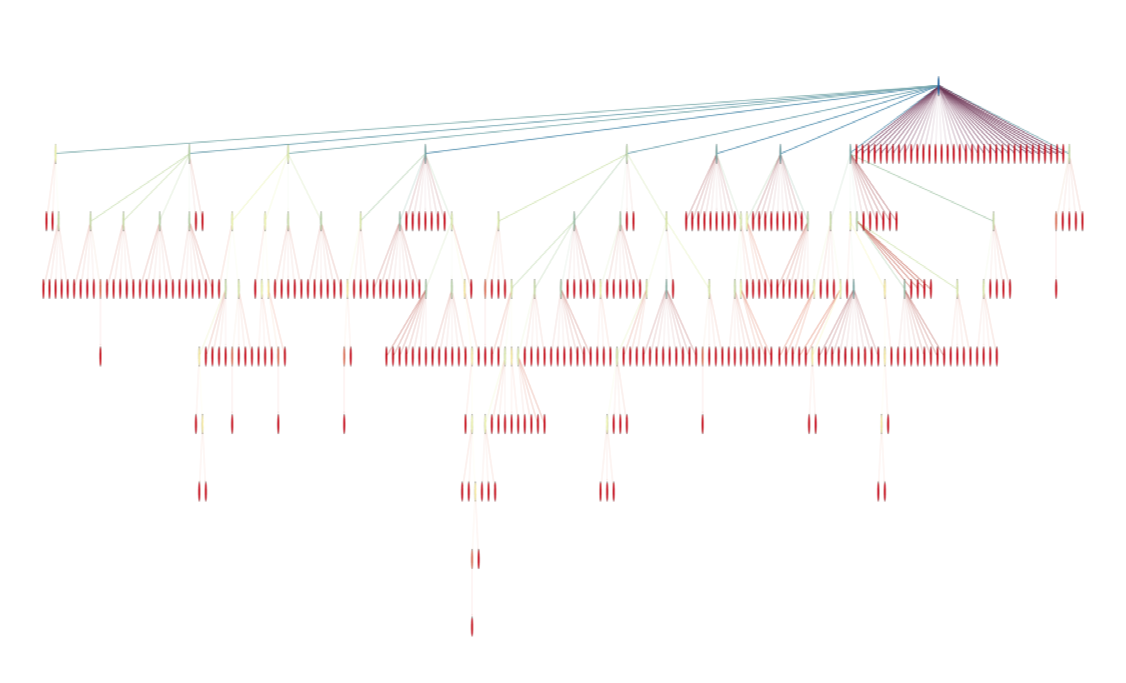
\includegraphics[scale=0.5]{Analysis/comms.png}
    \caption{Recursion Tree depicting how communities were found. The dataset was partitioned using the modularity algorithm. Partitions with more than 100 documents were then repartitioned recursively. Partitions of less than 100 documents were considered to be communities (shown red in the diagram). The figure shows the maximum depth of partition required was 8, and most communities were found after 3 partitions.}
\end{figure} 
\end{center}
Figure \ref{fig:COMMTREE} can be interpreted as the \emph{relationship} between different fields of research within the department. It is a shallow tree with highly branched nodes, suggesting that wide research fields, and qualitative overlap between fields.
The process described is equivalent to an unsupervised categorisation algorithm. The entire process, from model training to finding communities has been without human labelling or intuition. It was therefore instructive to examine what the algorithm defined as communities.
Communities were then analysed vigorously. Community clustering made intuitive sense in the majority of cases. Community 275 is typical:
\begin{table}[H]
\centering
\caption{Community 275}
\label{tabl:com275}
\begin{tabular}{||c|p{10cm}||}
\hline
Community Size                   & 15                                                                                                                                                                 \\ \hline
Depth down Recursion Tree        & 2                                                                                                                                                                  \\ \hline
Contents                         & Bees, Neonicotinoids, toxicology, pollen.                                                                                                                          \\ \hline
Article closest to Mean Vector                      & 10.1021/es2035152: Assessment of the Environmental Exposure of Honeybees to Particulate Matter Containing Neonicotinoid Insecticides Coming from Corn Coated Seeds \\ \hline
Community members                & (Some omitted for brevity)                                                                                                                                         \\ \hline
10.1007/s00216-012-6338-3        & UHPLC-DAD, method for the determination of neonicotinoid insecticides in single bees and, its relevance in honeybee colony loss investigations                     \\ \hline
10.1021/es2035152                & Assessment,of the Environmental Exposure of Honeybees to Particulate Matter Containing,Neonicotinoid Insecticides Coming from Corn Coated Seeds                    \\ \hline
10.1007/s11356-014-3470-y        & Systemic insecticides (neonicotinoids and fipronil): trends,uses,mode of action and metabolites                                                                    \\ \hline
10.1111/j.1439-0418.2012.01718.x & Aerial powdering of bees inside mobile cages and the extent of neonicotinoid cloud,surrounding corn drillers                                                       \\ \hline
10.1098/rsif.2013.0394           & Analysing photonic structures in plants                                                                                                                            \\ \hline
10.1007/s00114-013-1020-y        & The influence of pigmentation patterning on bumblebee foraging from flowers of Antirrhinum majus                                                                   \\ \hline
10.1111/ics.12035                & Keratins,and lipids in ethnic hair                                                                                                                                 \\ \hline
10.1021/ja047905n                & Photoluminescent,Layered Lanthanide Silicates                                                                                                                      \\ \hline
\end{tabular}
\end{table}

Table \ref{tab:com275} shows that this particular research community referes mainly to toxicology studies neonicotinoids,  bees and flowers\footnote{Note only some members of the community are shown above. Care was taken to give a representative sample of all 15 articles. The rest refer to Neonicotinoid insecticide studies with honey bees, and honey bee affinity to corn and pollen}. The connections mostly make sense. Note the surprising inclusion of the cosmetics and lanthanide silicate studies. Upon investigation, both studies use very similar analytical techniques used elsewhere in the community, and both examined intercalation.
\footnote{Both used made use of powder X-ray diffraction, and the silicates paper used thermogravimetry, the cosmetics study uses FID and several types of liquid chromatography, all methods used in the bee/nicotinoid studies.}

Note also that the mean vector for the community was closest to a paper in the training set that summarised the community extremely well. This paper could be considered as a \emph{Summary paper.}
The uses of this kind of analysis include:
\begin{itemize}
\item Analysis of literature field - plotting trees such as figure \ref{fig:COMMTREE} can give a relational understanding of how facets of a field link up together. 
\item Research tool: If researching a paper, finding its community immediately provides the researcher with papers that are related to it. Crucially this is done without simply following citations, so that interesting, perhaps overlooked links between papers can be found.
\item Summarising: If a researcher is required to read many papers from a field, they could find the communities involved and begin by reading the 'summary' papers. 
\end{itemize}

\section{Cambridge Staff Member Similarities}
\label{sec:AUTHORCLUSTERS}

It is not only articles themselves that can be grouped and analysed, but articles can be aggregated together to represent higher collections, such as staff members or research groups, or potentially even departments. 
To investigate this further, \texttt{http://www.ch.cam.ac.uk/publications/authors} was scraped in order to associate the documents in the CCD with particular staff members groups. A staff member vector $\textbf{f}$ was defined as $\mathbf{f}=\frac{1}{N}\sum_{i}^{N} \mathbf{v}_i$ , for an author with $N$ published articles in the CCD, with document vectors $\mathbf{v}_i$ (vector mean).

To investigate author relationships, a cosine matrix was created for each pair of authors A and B, with $\alpha$ and $\beta$ documents respectively, $\mathbf{C^{\left( A \right ) , \left( B \right)}}$ (see section\ref{sec:COSINEMAT}). The similarity between the author pair was defined as 
$$S_{A , B} = \sum_{i}^{\alpha} \sum_{j}^{\beta} C^{\left( A \right) , \left( B \right) }_{ i , j }$$
An Author similarity matrix can then be built up $\mathbf{S}$, with elements $\mathbf{S}_{ A , B }=S_{ A , B }$.
A similar technique could have been used to create clusters of authors. However, the sample size was now much smaller, so a more appropriate technique was hierarchical clustering, specifically UPGMA \footnote{Unweighted Pair Group Method with Arithmetic Mean} \cite{heatmapcluster}. This method clusters the authors pairwise in a hierarchical fashion.  An effective visualisation of the similarities between staff was to plot a \emph{clustermap} \cite{seaborn} \cite{scipy}.
\begin{center}
\begin{figure}[H]
\label{fig:AUTHORSIMS}
  \centering
    \includegraphics[scale=0.7]{Analysis/authorsims.png}
    \caption{This figure shows a heatmap of Author similarity. Dark pixels correspond to the author in the pixel's row having similar research interests to the author in the pixcel's column. The authors are arranged by clusters found in UPGMA of authors. The authors are also diagrammatically connected by a dendrogram. This shows the hierarchical structure of the clustering.}
\end{figure} 
\end{center}
Figure \ref{fig:AUTHORSIMS} shows the result of generating $\textbf{S}$ and performing a UPGMA hierarchical clustering. The authors are labelled by their crsids. The dendrogram tree links authors pairwise, illustrating how the clustering was performed, and how closely related clusters are. An enlarged dendrogram is shown below:
\begin{center}
\begin{figure}[H]
\label{fig:DENDRO}
  \centering
    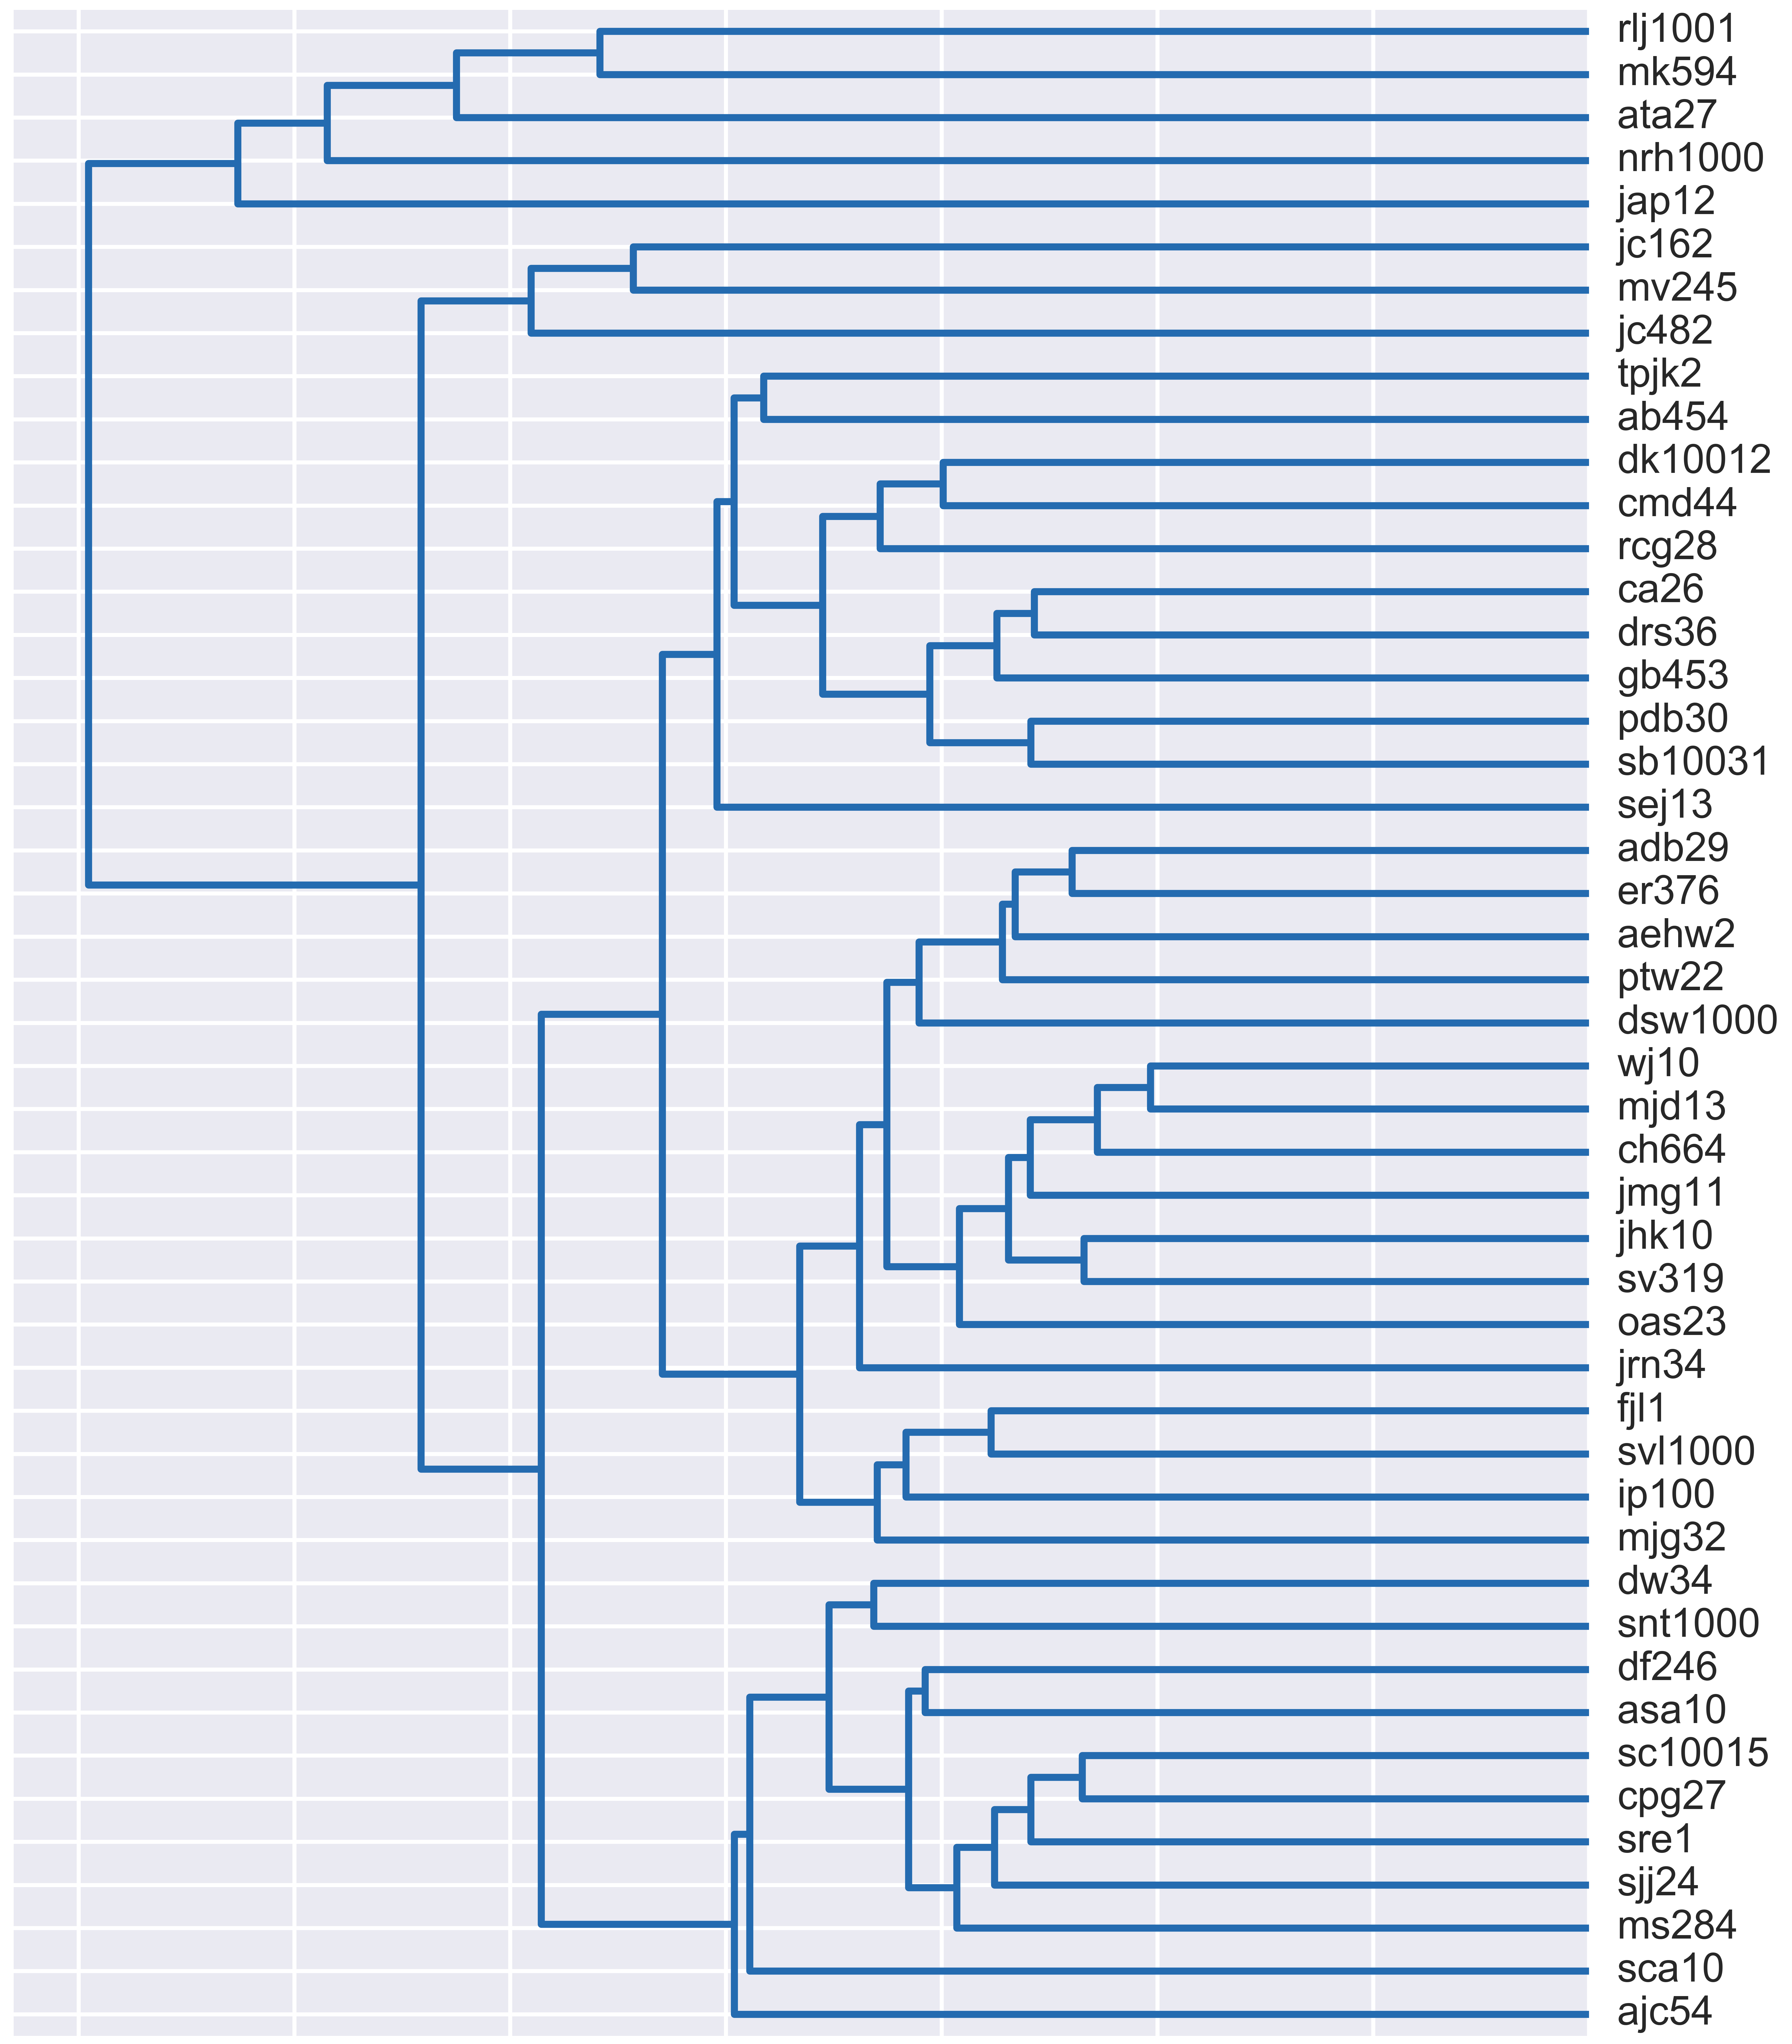
\includegraphics[scale=0.8]{Analysis/dendro.png}
    \caption{The dendrogram of figure \ref{fig:AUTHORSIMS}} plotted for clarity
\end{figure} 
\end{center}
A striking feature of figure \ref{fig:AUTHORSIMS} is the cluster in the bottom right corner. The dendrogram tree shows the members of this cluster occupy a separate branch of research space than the rest of the department. The staff members involved, Professor Jones, Dr. Harris, Professor Pyle Dr. Archibald and Dr. Kalberer are all members of the Centre for Atmospheric Science. The unsupervised model thus successfully `predicted' their department, and indicated that their work is quite far removed from most of the work in the Chemistry Department. This is a real success for the model. The dendrogram was then further examined and broken into distinct branches. Each branch was examined and manually labelled. The results are shown in figure \ref{sec:LABELLEDDENDRO}. Most clusters make intuitive sense, but there is one core of well connected, more disparate members (wj10 to jrn34). These members could be interpreted as being an interdisciplinary cluster.  
\begin{center}
\begin{figure}[H]
\label{fig:LABELLEDDENDRO}
  \centering
    \includegraphics[scale=0.8]{Analysis/dendro_overlay2.png}
    \caption{Cluster labels overlayed over the distinct branches of the dendrogram.}
\end{figure} 
\end{center}
The analysis's value is self evident. Clusters of similar staff members informs the department about the width of research (number of clusters), and how resources are partitioned (size of clusters). It should also be stressed that authors are associated without any human preconceptions or bias. Thus perhaps the most valuable author associations are the unexpected ones, and authors should be encouraged to examine their cluster and consider their `neighbours'.
\section{Combining research clusters and authors}
As a final data examination, topic communities found in section \ref{sec:RESEARCHCLUSTERS} were linked to the authors in the department. Different metrics for author similarity were developed to see if they correlated with the maps produced in the previous section.
Firstly, for a topic community $\mathfrak{C}$, with documents $d \in \mathfrak{C}$, and an author $\mathfrak{A}$ with documents $\delta \in \mathfrak{A}$, we can associate the author with the community if $\mathfrak{C} \cap \mathfrak{A} \neq \{ \}$, \footnote{or equivalently $\exists  \partial : \partial \in \mathfrak{C} \wedge \partial \in \mathfrak{A} $}. The function $f_{assoc}$ was defined as 
\[ 
f_{assoc}\left( \mathfrak{C} , \mathfrak{A} \right) = \begin{cases} 
      0 & \mathfrak{C} \cap \mathfrak{A} = \{ \} \\
      1 & \mathfrak{C} \cap \mathfrak{A} \neq \{ \} 
   \end{cases}
\]
It was noted that there was significant variation in the number of communities that researchers were associated with. A plot of $\sum_c^C f_{assoc} \left( \mathfrak{C}_c , \mathfrak{A} \right)$ for each author is shown below.:
\begin{center}
\begin{figure}[H]
\label{fig:commbar}
  \centering
    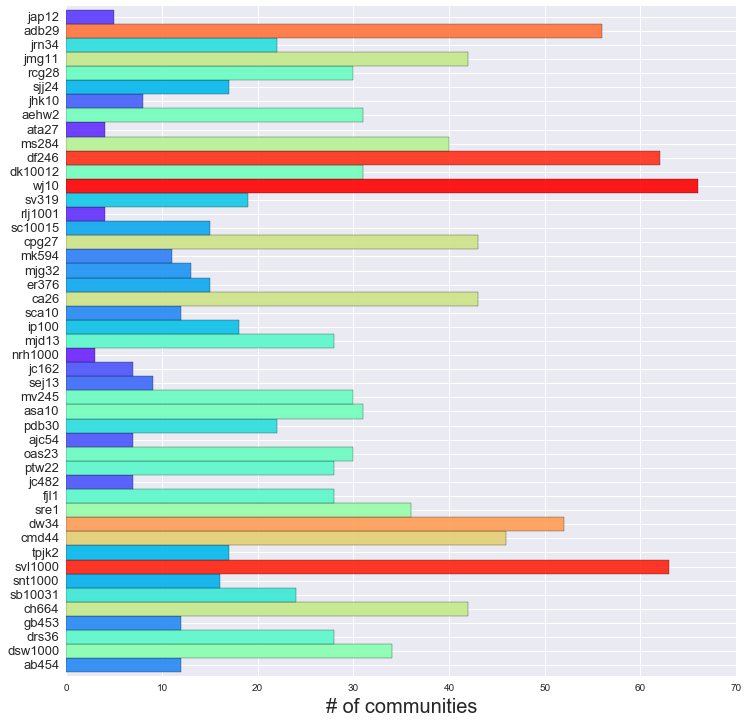
\includegraphics[scale=0.8]{Analysis/community_detection.png}
    \caption{Number of research communities authors are associated with. High values indicate an author publishing across many communities, suggest more interdisciplinary work, but also higher publication count per author. (The same plot, scaled for publication count) is included in the appendix}
\end{figure} 
\end{center}
It can be seen that some authors are widely distributed between communities, whereas others are concentrated.
It should be appreciated that communities are not uniformly distributed across work done in the department. For example there are many communities in `Life Sciences' but few in Atmospheric Chemistry, as such, interpretation of high values in Figure \ref{fig:commbar} corresponding 1:1 to wide research interests is cautious.

An association metric $S_{coincidence}$ between authors $\mathfrak{A}$ and $\mathfrak{B}$ was then defined as $$S_{coincidence}\left( \mathfrak{A} , \mathfrak{B} \right) = \sum_c^C \left(f_{assoc} \left( \mathfrak{C}_c , \mathfrak{A} \right) f_{assoc}\left( \mathfrak{C}_c , \mathfrak{B} \right) \right) $$
Where $C$ is the total number of communities. An association matrix was created, $\mathbf{S}^{Assoc}_{\mathfrak{A} , \mathfrak{B}} = S_{coincidence}\left( \mathfrak{A} , \mathfrak{B} \right)$, where high values for author pair $\mathfrak{A} , \mathfrak{B}$ indicate they appear in lots of research communities together. The matrix was then scaled such that: $\mathbf{S}^{Assoc,scaled}_{\mathfrak{A} , \mathfrak{B}} =  \mathbf{S}^{Assoc}_{\mathfrak{A} , \mathfrak{B}} /  \left( \mathbf{S}^{Assoc}_{\mathfrak{A} , \mathfrak{A}} + \mathbf{S}^{Assoc}_{\mathfrak{B} , \mathfrak{B}} \right) $, and normalised to the range 0,1. This was a measure of how often researchers can be found in the same communities. The matrix is shown below. 
\begin{center}
\begin{figure}[H]
\label{fig:commHEATMAP}
  \centering
    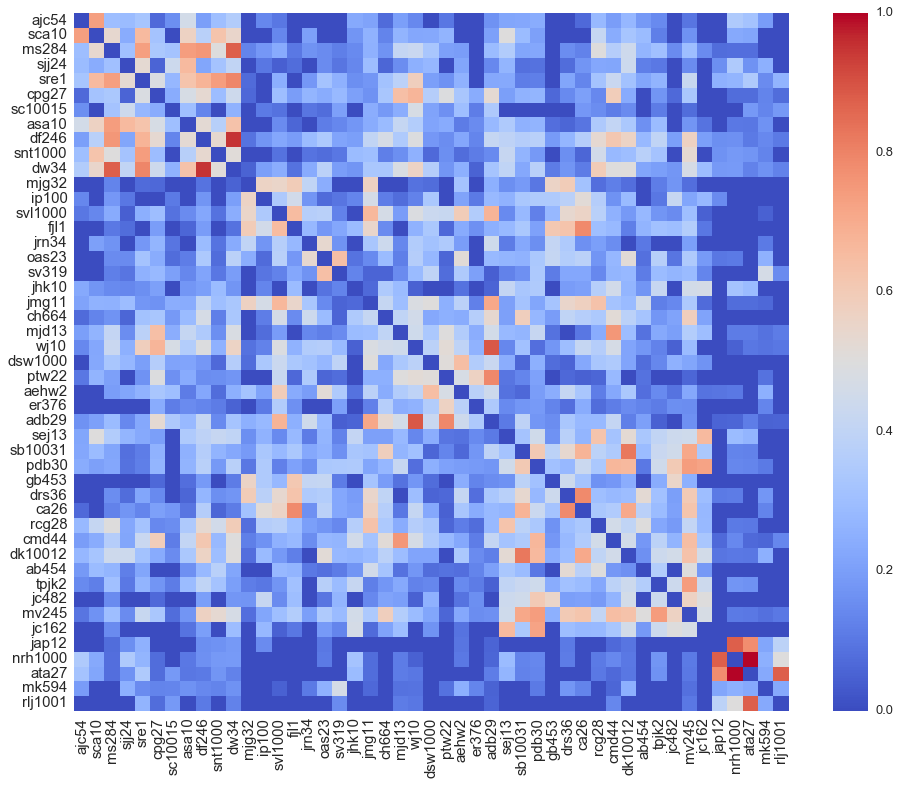
\includegraphics[scale=0.8]{Analysis/author_comm_heatmap.png}
    \caption{Heatmap showing author-author pair values for how often authors publish works in the same communities. High values indicated that Authors are predicted to have similar publication profiles. Note the authors are arranged with the ordering from figure \ref{fig:AUTHORSIMS}.}
\end{figure} 
\end{center}
Figure \ref{fig:commHEATMAP} indicates where authors have been detected to have similar research community occupations. High values should indicate that authors should ideally collaborate/communicate because they publish in the same research communities. Note also that the square patterns near the diagonal of the plot reproduce the clustering in figure \ref{fig:AUTHORSIMS}, lending weight to the validity of both analyses.\footnote{This is because the heatmap has been arranged according to the clustering found in section \ref{sec:AUTHORCLUSTERS}, but the matrix is derived in a completely different way (without applying any  clustering algorithm to the authors). Because clustering is qualitatively visible in figure \ref{fig:commHEATMAP}, there is a correlation between the two methods, i.e. they are consistent}.

Having defined a framework for finding where authors share research interest, the next step was to find where authors were \emph{actually} collaborating. It was possible to identify .... documents in CCD that were co-authored by staff members in the analysis. A heatmap for actual collaboration between authors is shown below, as well as a metric equivalent to the $\mathbf{S}^{Assoc,scaled}$ where elements are the sum of the number of communities both staff members have collaborated in.

\begin{figure}[H]
  \centering
  \begin{minipage}[b]{0.49\textwidth}
  \label{fig:rawcollabs}
    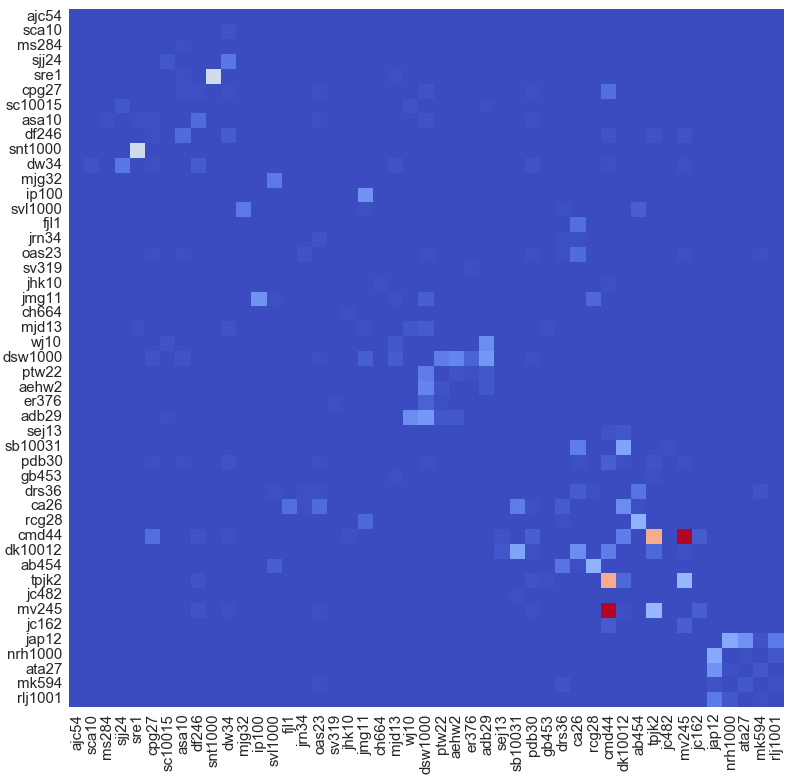
\includegraphics[width=\textwidth]{Analysis/raw_collabs.png}
    \caption{Raw collaboration matrix (values scaled to range 0,1). Note the general lack of co-publishing between staff members. Again staff are ordered by clustering described in section \ref{sec:AUTHORCLUSTERS}, but no actual clustering has been performed. Hot spots near the diagonal suggest that author pairs clustered together in \ref{sec:AUTHORCLUSTERS} generally collaborate more than distant author pairs.  }
  \end{minipage}
  \hfill
  \begin{minipage}[b]{0.49\textwidth}
  \label{fig:collcollabs}
    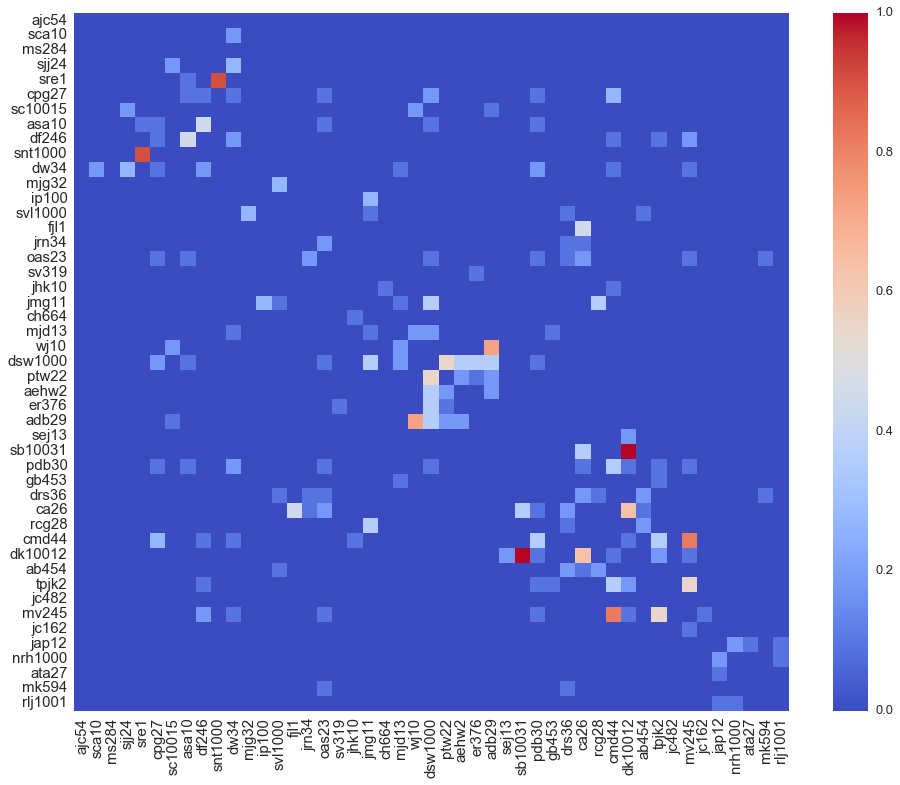
\includegraphics[width=\textwidth]{Analysis/comm_collabs.png}
    \caption{Matrix formed by summing collaboration of author pairs over research communities (values scaled to range 0,1). Qualitatively similar to \ref{fig:rawcollabs}. Hot spots near diagonal again suggest authors closely clustered in section \ref{sec:AUTHORCLUSTERS} collaborate more frequently }
  \end{minipage}
\end{figure}

Both pictures show the same qualitative picture. Similar author pairs (close to diagonal) are more likely to collaborate. 

As a final data treatment, a matrix defined as the difference between an author similarity matrix (e.g figures \ref{fig:AUTHORSIMS}, \ref{fig:commHEATMAP}) and an author collaboration matrix (e.g. figures \ref{fig:rawcollabs}, \ref{fig:collcollabs}) is interpretable as a \emph{recommended collaboration matrix}, i.e. where values close to 1 indicate high similarity but low collaboration, and values close to zero indicate effective collaboration and values close to -1 indicate high collaboration but low author similarity. Author Pairs with values to 1 should be encouraged to work together. This matrix is shown below:
\begin{center}
\begin{figure}[H]
\label{fig:RECOMM_MAT}
  \centering
    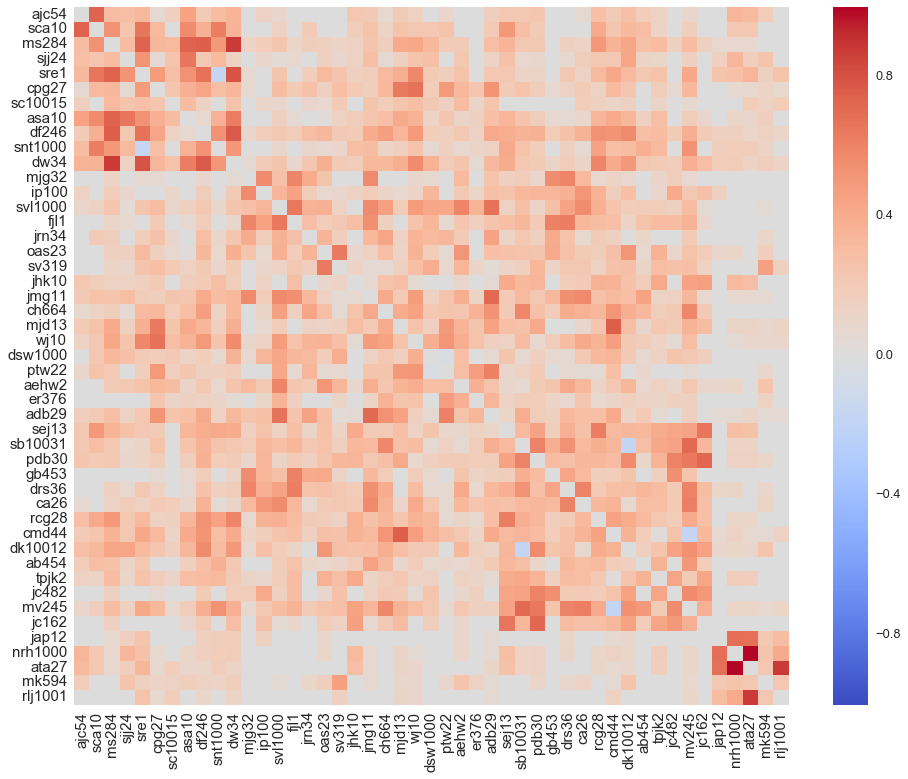
\includegraphics[scale=0.8]{Analysis/Recommending_Mat.png}
    \caption{Recommending matrix. High values (Deep red) indicate authors that have similar research but do not collaborate on published works. Values $\sim$ 0 (grey/white) are where authors are neither similar nor collaborate. Values towards -1, (Blue) indicate authors that are collaborate but do share similar research (not strongly observed, as expected. High negative values would be somewhat paradoxical.) }
\end{figure} 
\end{center}
This final piece of the analysis section illustrates how the framework developed over the research project reveals where it might be profitable for authors to collaborate. Returning to the Centre for Atmospheric Science, which was highlighted as a tight, separate research community, it can be seen that there are recommendations for greater collaboration between particular authors within the Centre. The matrix row for a particular staff member (Professor Goodman) is plotted below by way of example:
\begin{center}
\begin{figure}[H]
\label{fig:RECOMM_MAT}
  \centering
    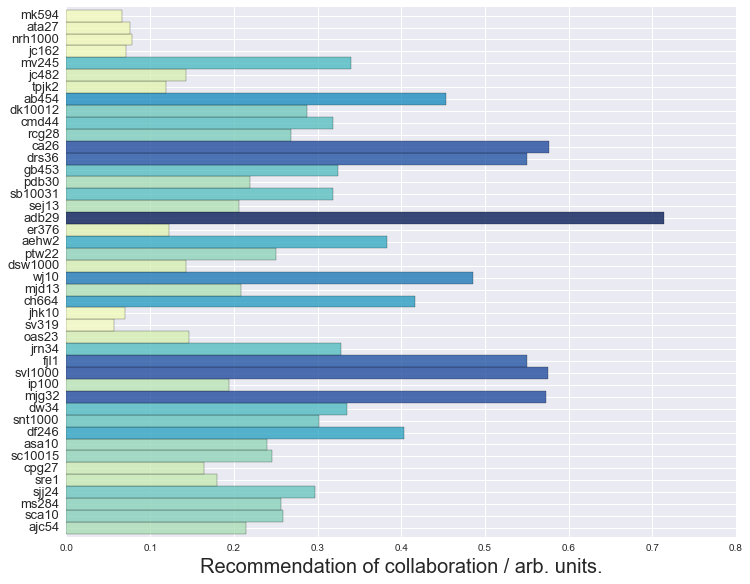
\includegraphics[scale=0.8]{Analysis/jmg.png}
    \caption{Recommendations for a particular staff member, Professor Goodman. (Bars very close to zero have been removed). }
\end{figure} 
\end{center}
The aim is that these maps and plots may trigger new, constructive debate and promote effective collaboration in the department. The analyses presented in this section are not exhaustive, and there is potential for more fruitful insights to be found. Please see section \ref{sec:RECOMMENDATIONS}


\chapter{Conclusions}
To Do
%\chapter{Recommendations for Further Work}
\label{chapt:RECOMMENDATIONS}
As alluded to in the text, there are several recommendations for further work. The code and data will be improved and amended over time, and is freely available under MIT licence on request \footnote{A digital copy is included with this dissertation.}. If attempting to carry out further work on this project, it is recommended to contact the author for in-depth explanations. This list is by no means exhaustive, and it is the author's belief that literature semantic analysis should be considered an important analytical chemical tool.
\section{Greater Dimensionality and Training Improvements}
The principles behind the methods discussed in the project have been shown to be sound. Models should now be improved. Computing resources should be obtained to train higher dimensional vectors \footnote{ The author recommends 400 dimensional vectors}. The models should also be trained for longer ($> 24$) epochs on more data ($> 460000$ documents). These steps will lead to more expressive models.
\section{Greater use of word vectors}
This project focussed mainly on document vectors. However word vectors may be very useful. A method for testing the quality of improved models should be developed. This could take the form of expected relationships to test the model. E.g. Fluorine is to Fluoride as Chlorine is to ... . Many hundreds of these relationships should be systematically built up to test model intuition.\footnote{This would probably require much larger, more descriptive training sets, e.g. textbook transcipts etc.} This follows the methodologies set out in the literature \cite{word2vec1} \cite{word2vec2}. Furthermore, is is possible to predict chemical properties using semantic relationships found in the literature? Vec(Compound A) + Vec(Compound B) + Vec(Lab Technique) may give vec(Product C). If so, it may be possible to find unexpected reactions. This could be coupled with the RInChI database to form a new type of data-driven cheminformatics.
\section{Time resolution in clustering}
Methods have been described for clustering documents. The cluster centres represent the content of the cluster effectively. By finding early papers in the cluster, is it possible to identify influential papers or authors?
By clustering on documents from particular years, is it possible to identify a path for the evolving cluster centre vector? If so, it should be possible to extrapolate to \emph{predict} near future research directions.
\section{Open Source Chemistry Vectors}
With the increase in open source papers, it should be possible to build up a vast dataset of chemical language for training using the bodies of articles published on open source platforms, and even to use supplied supporting information. 
\section{Structure stemming}
Chemical names could be smartly preprocessed to classes of chemicals e.g. by identifying a compound from its name and mapping to InChI key, then to a chemical class. This would allow better association of chemical fragments in training.
\section{Multiply labelled Documents}
In Training Doc2Vec, by specifying document with more than just their unique identifiers allows more vectors to be associated. By identifying and labelling all documents with a particular concept, e.g. 'palladium-catalysed', and then training Doc2Vec, one defines an 'palladium-catalysed' vector, specifically trained for the concept. These concept vectors would be robust and information rich\footnote{For example, which documents are close to the indium-catalysed vector but do not contain the word indium...}

%\bibliography{References}
%\chapter{Appendix}
\section{UK Departments scraped}
\begin{table}[H]
\begin{tabular}{||p{2.5cm}|Y||}
\hline
 Department                         & URL \\
\hline
 \footnotesize{Aberdeen                       }    & \footnotesize{\url{http://www.abdn.ac.uk/chemistry/}}                                                                                                     \\
 \footnotesize{Aston                         }     & \footnotesize{\url{http://www.aston.ac.uk/eas/about-eas/academic-groups/ceac/}}                                                                           \\
 \footnotesize{Bangor                       }      & \footnotesize{\url{http://www.bangor.ac.uk/chemistry/index.php}}                                                                                          \\
 \footnotesize{Bath                        }       & \footnotesize{\url{http://www.bath.ac.uk/chemistry/}}                                                                                                     \\
 \footnotesize{Belfast (Queen's)          }        & \footnotesize{\url{http://www.qub.ac.uk/schools/SchoolofChemistryandChemicalEngineering/}}                                                                \\
\footnotesize{Birmingham                }         & \footnotesize{\url{http://www.birmingham.ac.uk/schools/chemistry/index.aspx}}                                                                             \\
\footnotesize{Bradford                 }          & \footnotesize{\url{http://www.brad.ac.uk/acad/chemistry/}                                                                                               } \\
 \footnotesize{Brighton                }           & \footnotesize{\url{http://about.brighton.ac.uk/pharmacy/}}                                                                                                \\
 \footnotesize{Bristol                }            & \footnotesize{\url{http://www.bris.ac.uk/Depts/Chemistry/Bristol\_Chemistry.html}}                                                                         \\
 \footnotesize{Cambridge             }             & \footnotesize{\url{http://www.ch.cam.ac.uk/}}                                                                                                             \\
 \footnotesize{Cardiff              }              & \footnotesize{\url{http://www.cardiff.ac.uk/chemistry}}                                                                                                   \\
 \footnotesize{Dundee              }               & \footnotesize{\url{http://www.lifesci.dundee.ac.uk}}                                                                                                      \\
 \footnotesize{Durham             }                & \footnotesize{\url{http://www.dur.ac.uk/chemistry/}}                                                                                                      \\
 \footnotesize{Edinburgh         }                 & \footnotesize{\url{http://www.chem.ed.ac.uk/}}                                                                                                            \\
 \footnotesize{Essex            }                  & \footnotesize{\url{http://www.essex.ac.uk/bs/}                                                                                                          } \\
 \footnotesize{Glasgow         }                   & \footnotesize{\url{http://www.chem.gla.ac.uk/}}                                                                                                           \\
 \footnotesize{Greenwich      }                    & \footnotesize{\url{http://www.gre.ac.uk/engsci/study/pharchemenv}}                                                                                        \\
 \footnotesize{Heriot-Watt   }                     & \footnotesize{\url{http://www.eps.hw.ac.uk/institutes/chemical-sciences.htm}}                                                                             \\
 \footnotesize{Hertfordshire}                      & \footnotesize{\url{http://www.herts.ac.uk/research/hhsri/research-areas-hhsri/pharmacy-and-pharmacology/pharmaceutical-chemistry}}                        \\
 \footnotesize{Huddersfield}                       & \footnotesize{\url{http://www.hud.ac.uk/sas/chemistry/}}                                                                                                  \\
 \footnotesize{Hull       }                        & \footnotesize{\url{http://www2.hull.ac.uk/science/chemistry.aspx}}                                                                                        \\
 \footnotesize{Keele     }                         & \footnotesize{\url{http://www.keele.ac.uk/chemistry/}}                                                                                                    \\
 \footnotesize{Kent at Canterbury}                 & \footnotesize{\url{http://www.kent.ac.uk/bio/}}                                                                                                           \\
 \footnotesize{Kingston     }                      & \footnotesize{\url{http://sec.kingston.ac.uk/research/research-centres/}}                    
 \\
 \footnotesize{Lancaster   }                       & \footnotesize{\url{http://www.lancaster.ac.uk/chemistry/}}                                                                                                \\\
\footnotesize{Leeds      }                        & \footnotesize{\url{http://www.chem.leeds.ac.uk/}}                                                                                                         \\
 \footnotesize{Leicester }                         & \footnotesize{\url{http://www.le.ac.uk/chemistry/}}                                                                                                                                                               
\\
\hline 
 \end{tabular}
 \end{table}
 
 \begin{table}[H]
 \begin{tabular}{||p{4cm}|Y||}
\hline
 Department                         & URL \\
\hline
 \footnotesize{Lincoln                        }    & \footnotesize{\url{https://www.lincoln.ac.uk/home/chemistry/}}                                                                                            \\
 \footnotesize{Liverpool                     }     & \footnotesize{\url{http://www.liv.ac.uk/chemistry/}}                                                                                                      \\
 \footnotesize{Liverpool John Moores        }      & \footnotesize{\url{https://www.ljmu.ac.uk/about-us/faculties/faculty-of-science/school-of-pharmacy-and-biomolecular-sciences}}                            \\
 \footnotesize{London Met.         }       & \footnotesize{\url{http://www.londonmet.ac.uk/faculties/faculty-of-life-sciences-and-computing/school-of-human-sciences/}}                                \\
 \footnotesize{Loughborough               }        & \footnotesize{\url{http://www.lboro.ac.uk/departments/chemistry}}                                                                                         \\
 \footnotesize{Manchester                }         & \footnotesize{\url{http://www.manchester.ac.uk/chemistry/}}                                                                                               \\
 \footnotesize{Manchester Met.  }          & \footnotesize{\url{http://www.sste.mmu.ac.uk}}                                                                                                            \\
 \footnotesize{Newcastle  }                        & \footnotesize{\url{http://www.ncl.ac.uk/chemistry/}}                                                                                                      \\
 \footnotesize{Northumbria}                        & \footnotesize{\url{https://www.northumbria.ac.uk/about-us/academic-departments/applied-sciences/}}\\
 \footnotesize{Nottingham                  }       & \footnotesize{\url{http://www.nottingham.ac.uk/chemistry/}}                                                                                               \\
 \footnotesize{Nottingham Trent}        & \footnotesize{\url{http://www.ntu.ac.uk/sat/about/academic\_teams/chemistry.html}}                                                                         \\
\footnotesize{ Open University }                   & \footnotesize{\url{http://www.open.ac.uk/science/chemistry/}}                                                                                             \\
 \footnotesize{Oxford}                             & \footnotesize{\url{http://www.chem.ox.ac.uk/}}                                                                                                            \\
 \footnotesize{Univ. West Scotland} & \footnotesize{\url{http://www.uws.ac.uk/schools/school-of-science/departments/chemistry-and-chemical-engineering/}}                                       \\
 \footnotesize{Plymouth               }            & \footnotesize{\url{https://www.plymouth.ac.uk/schools/school-of-geography-earth-and-environmental-sciences/chemistry}}                                    \\
\footnotesize{Reading               }             & \footnotesize{\url{http://www.reading.ac.uk/chemistry/}}                                                                                                  \\
 \footnotesize{Robert Gordon        }              & \footnotesize{\url{http://www.rgu.ac.uk/about/faculties-schools-and-departments/faculty-of-health-and-social-care/school-of-pharmacy-and-life-sciences1}} \\
 \footnotesize{St Andrews          }               & \footnotesize{\url{http://ch-www.st-and.ac.uk/}}                                                                                                          \\
 \footnotesize{Salford            }                & \footnotesize{\url{http://www.salford.ac.uk/environment-life-sciences/research/biomedical}}                                                               \\
 \footnotesize{Sheffield         }                 & \footnotesize{\url{http://www.sheffield.ac.uk/chemistry}}                                                                                                 \\
 \footnotesize{Sheffield Hallam }                  & \footnotesize{\url{http://www.shu.ac.uk/schools/sci/chem/}}                                                                                               \\
 \footnotesize{South Wales  }                      & \footnotesize{\url{http://www.southwales.ac.uk/chemistry/}}                                                                                               \\
 \footnotesize{Southampton }                       & \footnotesize{\url{http://www.soton.ac.uk/chemistry/}}                                                                                                    \\
 \footnotesize{Strathclyde}                        & \footnotesize{\url{http://www.strath.ac.uk/chemistry/}}                                                                                                   \\
 \footnotesize{Sunderland}                         & \footnotesize{\url{http://www.sunderland.ac.uk/ug/subjectareas/pharmacychemistrybiomedicalsciences/}}                                                     \\
 \footnotesize{Surrey }                            & \footnotesize{\url{http://www.surrey.ac.uk/chemistry/}}                                                                                                   \\
 \footnotesize{Sussex                            } & \footnotesize{\url{http://www.sussex.ac.uk/chemistry/}}                                                                                                   \\
 \footnotesize{Teesside                         }  & \footnotesize{\url{http://www.tees.ac.uk/schools/sst/}}                                                                                                   \\
 \footnotesize{UEA                             }   & \footnotesize{\url{http://www.uea.ac.uk/chemistry}}                                                                                                       \\
 \footnotesize{Warwick                        }    & \footnotesize{\url{http://www2.warwick.ac.uk/fac/sci/chemistry/}}                                                                                         \\
 \footnotesize{York                          }     & \footnotesize{\url{http://www.york.ac.uk/depts/chem/}}                                                                                                   \\ \hline
\end{tabular}
\end{table}


\begin{table}[H]
\begin{tabular}{||p{4cm}|Y||}
\hline
Department                         & URL \\
\hline
 \footnotesize{Bradford Ploymer IRC         }      & \footnotesize{\url{http://www.brad.ac.uk/acad/irc/}}                                                                                                      \\
 \footnotesize{Cardiff Pharmacy            }       & \footnotesize{\url{http://www.cardiff.ac.uk/pharmacy-pharmaceutical-sciences}}                                                                            \\
 \footnotesize{Burbeck Chemistry          }        & \footnotesize{\url{http://www.bbk.ac.uk/bcs/}}                                                                                                            \\
 \footnotesize{Burbeck Crystallography   }         & \footnotesize{\url{http://www.cryst.bbk.ac.uk/}}                                                                                                          \\
 \footnotesize{Imperial College London  }          & \footnotesize{\url{http://www.imperial.ac.uk/chemistry/}}                                                                                                 \\
 \footnotesize{King's College London   }           & \footnotesize{\url{http://www.kcl.ac.uk/nms/depts/chemistry/index.aspx}}                                                                                  \\
 \footnotesize{Queen Mary London      }            & \footnotesize{\url{http://www.sbcs.qmul.ac.uk/}}                                                                                                          \\
 \footnotesize{UCL School of Pharmacy}             & \footnotesize{\url{http://www.ucl.ac.uk/pharmacy}}                                                                                                        \\
 \footnotesize{University College London}          & \footnotesize{\url{http://www.ucl.ac.uk/chemistry/}}                                                                                                      \\
 \footnotesize{Sheffield Comput. Chem.}  & \footnotesize{\url{http://www.sheffield.ac.uk/is/research/groups/chemoinformatics}}                                                                       \\
\hline
\end{tabular}
\end{table}
\section{Publishers Considered in UK scraping}
\begin{table}[H]
\centering
\begin{tabular}{||c||}
\hline
Publishers collected in UK scraping run \\
\hline 
IBM                                               \\
Pleiades Publishing Ltd                           \\
Informa Healthcare                                \\
Informa UK Limited                                \\
Royal Society of Chemistry (RSC)                  \\
Vilnius Gediminas Technical University            \\
Technical Association of Photopolymers, Japan     \\
Springer US                                       \\
Trans Tech Publications                           \\
Thieme Publishing Group                           \\
Nature Publishing Group                           \\
American Physical Society (APS)                   \\
IOP Publishing                                    \\
Institute of Electrical \& Electronics Engineers (IEEE)\\
American Chemical Society (ACS)                   \\
Walter de Gruyter GmbH                            \\
Pharmaceutical Society of Japan                   \\
American Association of Physics Teachers (AAPT)   \\
AIP Publishing                                    \\
Japan Society of Applied Physics                  \\
American Vacuum Society                           \\
Wiley-Blackwell                                   \\
Springer Berlin Heidelberg                        \\
Springer New York                                 \\
Royal Society of Chemistry                        \\
Public Library of Science (PLoS)                  \\
Surface Science Society Japan                     \\
Springer Science + Business Media                 \\
The Royal Society                                 \\
Society of Rheology                               \\
Acoustical Society of America (ASA)               \\
Springer International Publishing                 \\
Proceedings of the National Academy of Sciences   \\
Japan Society for Analytical Chemistry            \\
International Union of Crystallography (IUCr)     \\
Chemical Society of Japan                         \\
EDP Sciences                                      \\
\hline
\end{tabular}
\end{table}
\section{Scaled Communities for staff members in Cambridge}
\begin{center}
\begin{figure}[H]
\label{fig:LABELLEDDENDRO}
  \centering
    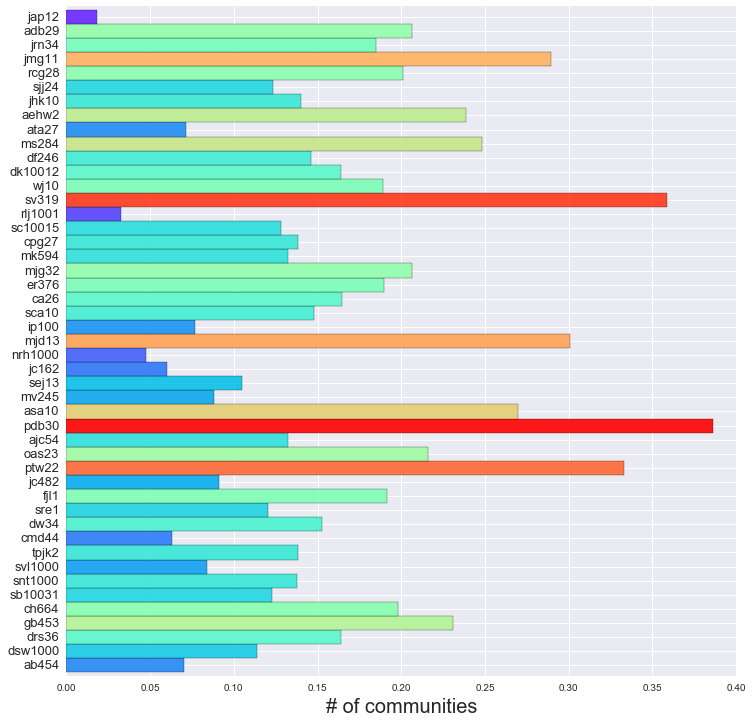
\includegraphics[width=\textwidth]{Analysis/community_detection2.png}
    \caption{Number of research communities authors are associated with. High values suggest more interdisciplinary work. The bars have been scaled relative to the author's total publication count. }
\end{figure} 
\end{center}
\end{document}  